\documentclass{doku2018}
\usepackage[utf8]{inputenc}
\usepackage[ngerman]{babel}
\usepackage{blindtext}
\usepackage{amsmath,amssymb,amsthm,amstext}
\usepackage{asymptote}
\usepackage{listings}
\usepackage{graphicx}
\usepackage{tikz}
\usepackage{bookmark}
\usepackage{hyperref}
\usetikzlibrary{graphs, shapes, arrows, snakes, positioning, fit}
\lstset{literate=%
  {Ö}{{\"O}}1
  {Ä}{{\"A}}1
  {Ü}{{\"U}}1
  {ß}{{\ss}}1
  {ü}{{\"u}}1
  {ä}{{\"a}}1
  {ö}{{\"o}}1
}
\tikzstyle{block} = [rectangle, draw, fill=blue!20, 
    text width=5em, text centered, rounded corners, minimum height=4em]
\tikzstyle{line} = [draw, -latex']
\tikzstyle{cloud} = [draw, ellipse,fill=red!20, node distance=3cm,
    minimum height=4em, minimum width=4em]
\newcommand\wichtig[1]{\textbf{#1}}
\usepackage{hologo} % für LaTeX-Logos
%\usepackage{TheSansOsF}
\newtheorem{df}{Definition}
\newtheorem{satz}{Satz}
\newtheorem{fakt}{Fakt}
\newtheorem{lemma}{Lemma}
\newtheorem{korollar}{Korollar}

\academy{Akademie Grovesmühle}{2018}{3}


%%%Die folgenden 5 Befehle werden zum Zeichnen der Kugel mit dem Graphen auf der Oberfläche benötigt:
\newcommand\pgfmathsinandcos[3]{
  \pgfmathsetmacro#1{sin(#3)}
  \pgfmathsetmacro#2{cos(#3)}
}
\newcommand\LongitudePlane[3][current plane]{
  \pgfmathsinandcos\sinEl\cosEl{#2}
  \pgfmathsinandcos\sint\cost{#3}
  \tikzset{#1/.style={cm={\cost,\sint*\sinEl,0,\cosEl,(0,0)}}}
}
\newcommand\LatitudePlane[3][current plane]{
  \pgfmathsinandcos\sinEl\cosEl{#2}
  \pgfmathsinandcos\sint\cost{#3}
  \pgfmathsetmacro\yshift{\cosEl*\sint}
  \tikzset{#1/.style={cm={\cost,0,0,\cost*\sinEl,(0,\yshift)}}}
}
\newcommand\DrawLongitudeCircle[2][1]{
  \LongitudePlane{\angEl}{#2}
  \tikzset{current plane/.prefix style={scale=#1}}
  \pgfmathsetmacro\angVis{atan(sin(#2)*cos(\angEl)/sin(\angEl))}
  \draw[current plane] (\angVis:1) arc (\angVis:\angVis+180:1);
  \draw[current plane,dashed] (\angVis-180:1) arc (\angVis-180:\angVis:1);
}
\newcommand\DrawLatitudeCircle[2][1]{
  \LatitudePlane{\angEl}{#2}
  \tikzset{current plane/.prefix style={scale=#1}}
  \pgfmathsetmacro\sinVis{sin(#2)/cos(#2)*sin(\angEl)/cos(\angEl)}
  \pgfmathsetmacro\angVis{asin(min(1,max(\sinVis,-1)))}
  \draw[current plane] (\angVis:1) arc (\angVis:-\angVis-180:1);
  \draw[current plane,dashed] (180-\angVis:1) arc (180-\angVis:\angVis:1);
}%%%

\definecolor{black}{RGB}{0, 0, 0}

\begin{document}
\tableofcontents

 \course[Baum Wald Fluss]{Baum Wald Fluss}{1}{\includegraphics[width=.9\textwidth]{img/Titelbild-neu.png}}
\section{Aus der Kursbeschreibung}
\authors{Markus Oehme und Sebastian Brandt}

Bei Gelegenheit könnte hier Inhalt stehen.\cite[s. Literaturverzeichnis]{quelle1}



\section{Graphen}
\authors{Jakob Gierschmann und Annika Dunkel}

\subsection{Was sind Graphen?}
\begin{figure}
\centering
	\begin{tikzpicture}
	\node[draw, circle](a) at (1,0){a};
	\node[draw, circle](b) at (1,2){b};
	\node[draw, circle](c) at (2,3){c};
	\node[draw, circle](d) at (3,2){d};
	\node[draw, circle](e) at (3,0){e};
	\node[draw, circle](f) at (5,2){f};
	\draw (a) -- (b);
	\draw (b) -- (d);
	\draw (c) -- (b);
	\draw (c) -- (d);
	\draw (d) -- (f);
	\draw (d) -- (e);
	\draw (a) -- (e);
	\end{tikzpicture}
	\caption{Ein Graph}
	\label{einfuehrungsgraph}
\end{figure}

Ein \wichtig{Graph} besteht aus \wichtig{Knoten} und \wichtig{Kanten}.  
Abb. \ref{einfuehrungsgraph} zeigt ein einfaches Beispiel für einen Graphen.


\begin{df}
Ein Graph ist ein Tupel $G = (V,E)$ aus einer endlichen Knotenmenge $V$ und einer Kantenmenge $E \subseteq \{e \in 2^{V}\mid |e| = 2\}$.
\end{df}

\subsection{Geschichte der Graphentheorie}
\textit{Leonhard Euler} (1707--1783) wird im Allgemeinen als Begründer der Graphentheorie bezeichnet. Er befasste sich mit Problemstellungen wie dem \wichtig{Königsberger Brückenproblem}.
Auch wenn er bereits die ersten Konzepte der Graphentheorie auf aufstellte, entwickelte sich die Graphentheorie in den folgenden 100 Jahren kaum weiter. 
Erst \textit{Gustav Robert Kirchhoff} (1824--1887), der elektrische Ströme mithilfe der Graphentheorie darstellte, ermöglichte dadurch den nächsten großen Durchbruch.
Schließlich brachte \textit{Arthur Cayley} (1821--1895)  die Strukturformeln von chemischen Molekülen in die Graphentheorie ein. Außerdem stellte er den \wichtig{Vierfarbensatz} auf.
Ab 1945 machte die Graphentheorie aufgrund der rasanten Computerentwicklung noch größere Fortschritte.

\subsection{Teilgraphen}
	Ein Teilgraph $G'$ besteht aus einem Teil der Knoten und Kanten eines übergeordneten Graphen $G$.
	\begin{df}
	Ein Graph $ G' = (V', E')$ ist ein Teilgraph von $G = (V, E)$, wenn $V' \subseteq V$ und $E' \subseteq E$, sodass für alle $e = \{v_1, v_2\} \in E'$ auch $v_1, v_2 \in V'$.
	\end{df}
	\begin{df}
	Ein Teilgraph $ G' = (V', E')$ von $G = (V, E)$ heißt von $V'$ induzierter Teilgraph, wenn jede Kante $e \in E$ , die zwischen Knoten $v'_1,v'_2 \in V'$ verläuft, auch in $E'$ vorhanden ist.
	\end{df}

\subsection{Verbindungen}
Graphen haben einige wichtige Eigenschaften, die wir im Folgenden beschreiben und definieren wollen.



\begin{df}
Ein Weg der Länge n ist eine Folge von Knoten $v_0,v_1, v_2, \dotsc, v_n \in V$, sodass Kanten $e = \{v_{i-1},v_i\} \in E$ für $ 1 \leq i \leq n$ existieren.
\end{df}

\begin{df}
Ein Pfad ist ein Weg, bei dem alle Knoten paarweise verschieden sind.
$v_0$ heißt Startknoten und $v_n$ heißt Zielknoten.
\end{df}

\begin{df}
Ein Graph $G = (V,E)$ heißt zusammenhängend, wenn zu je zwei Knoten $v_1, v_2 \in V$ein Pfad von $v_1$ nach $v_2$ existiert.
\end{df}

\begin{df}
Die maximalen zusammenhängenden Teilgraphen heißen Zusammenhangskomponenten.
\end{df}

\subsection{Variationen}

Neben den gewöhnlichen Graphen gibt es einige \wichtig{Variationen}, die in der Regel ausdrücklich als solche gekennzeichnet werden.


\begin{itemize}
\item \wichtig{Multigraphen} Ein  Multigraph lässt mehrere Kanten statt nur einer Kante zwischen zwei Knoten zu.
\item \wichtig{Gerichteter Graphen} Bei einem gerichteten Graphen sind die Kanten keine Mengen, sondern Tupel. Die Knoten, die sie verbinden haben also eine Reihenfolge und somit hat die Kante eine feste Richtung.
\item \wichtig{Graphen mit Schleifen}  Wenn ein Knoten durch eine Kante mit sich selbs verbundn ist, ist diese Kante eine Schleife. In Graphen, die Schleifen zulassen, ist also ist $|e| = 1$ zulässig.
\item \wichtig{Unendliche Graphen} Wenn Graphen eine unendliche Anzahl von Knoten $V$ und/oder Kanten  $E$ haben, werden sie unendliche Graphen genannt.
\end{itemize}

\subsection{Spezielle Graphen}
In der Graphentheorie gibt es spezielle Graphen, die besondere Eigenschaften haben. Einige von ihnen nennen wir kurz, um uns später auf sie beziehen zu können.


\begin{figure}
	\centering
	\begin{tikzpicture}
	\node[draw, circle](a) at (0,0){a};
	\node[draw, circle](b) at (2,0){b};
	\node[draw, circle](c) at (0,2){c};
	\node[draw, circle](d) at (2,2){d};
	\draw(a) -- (b);
	\draw(a) -- (c);
	\draw(a) -- (d);
	\draw(b) -- (c);
	\draw(b) -- (d);
	\draw(c) -- (d);
	\end{tikzpicture}
	
	\caption{Der Graph $K_4$}
	\label{k4}
\end{figure}

\begin{figure}
	\centering
	\begin{tikzpicture}
	\node[draw, circle](a) at (0.0:2){a};
	\node[draw, circle](b) at (72.0:2){b};
	\node[draw, circle](c) at (144.0:2){c};
	\node[draw, circle](d) at (216.0:2){d};
	\node[draw, circle](e) at (288.0:2){e};
	\draw(a) -- (b);
	\draw(b) -- (c);
	\draw(c) -- (d);
	\draw(d) -- (e);
	\draw(e) -- (a);
	\end{tikzpicture}
	\caption{Der Graph $C_5$}
	\label{c5}
\end{figure}

\begin{figure}
	\centering
	\begin{tikzpicture}
	\node[draw, circle](a) at (1,0){a};
	\node[draw, circle](b) at (1,1){b};
	\node[draw, circle](c) at (0,2){c};
	\node[draw, circle](d) at (2,2){d};
	\node[draw, circle](e) at (4,0){e};
	\node[draw, circle](f) at (4,1){f};
	\node[draw, circle](g) at (3,2){g};
	\node[draw, circle](h) at (5,2){h};
	\node[draw, circle](i) at (5,1){i};
	\draw(a) -- (b);
	\draw(b) -- (c);
	\draw(b) -- (d);
	\draw(e) -- (f);
	\draw(f) -- (g);
	\draw(f) -- (h);
	\draw(e) -- (i);

	\end{tikzpicture}
	\caption{Ein Wald aus zwei Bäumen}
	\label{wood}
\end{figure}
\begin{df}
Ein vollständiger Graph $K_n$ ist ein Graph $G = (V,E)$ mit $n$ Knoten, bei dem je zwei Knoten $v,w \in V$ durch eine Kante $ e = \{v,w\} $ verbunden sind.
\end{df}
Ein Beispiel für einen vollständigen Graphen ist der Graph $K_4$ in Abb. \ref{k4}.
\begin{df}
Ist $v_0,v_1,\dotsc,v_n$ ein Pfad und existiert $e_0 = \{v_n, v_o\}$ so ist $v_0, v_1, \dotsc, v_n$ ein Kreis. Einen Kreis mit $n$ Knoten nennen wir $C_n$.
\end{df}
Ein Beispiel für einen Kreis ist der Graph $C_5$ in Abb. \ref{c5}.
\begin{df}
Ein Wald ist ein Graph ohne Kreise. Die Zusammenhangskomponenten heißen Bäume.
\end{df}
Abb. \ref{wood} zeigt ein Beispiel für einen Wald.





\subsection{Wichtige Messgrößen}
Es gibt in Graphen einige Meßgrößen, die wir durch Funktionen oder Variablen angeben können. Einige seien hier kurz definiert.\\

Der Grad eines Knotens ist ein Beispiel für eine lokale Messgröße, da wir ihn beschreiben können, ohne den ganzen Graphen zu betrachten.
\begin{df}
Sei $v \in V$ ein Knoten.
Der Grad von $v$, geschrieben $d(v)$, ist die Anzahl an Kanten, die $v$ enthalten.
\begin{center}
$d(v) := |\{e \in E \mid v \in e\}|$
\end{center}
\end{df}

\begin{df}
Das Minimum aller Grade der Knoten $v \in V$ wird mit $\delta$ bezeichnet, das Maximum mit $\Delta$.
\end{df}

\begin{fakt}
Die Summe $\sum\limits_{v\in V}d(v)$ ist gerade und $|E|  = \frac{1}{2}\sum\limits_{v\in V}d(v)$.
\begin{proof}
Jede Kante verbindet zwei Knoten, also erhöht jede Kante die Summe aller Grade um 2.
\end{proof}
\end{fakt}

Mit den gerade definierten Eigenschaften von Graphen können wir eine weitere Funktion einführen, die wir benutzen können, um Knoten besser differenzieren zu können.

\begin{df}
Der Abstand $d(v,v')$ zwischen zwei Knoten $v,v' \in V$ ist die Länge des kürzesten Pfades von $v$ nach $v'$. Gibt es keinen solchen Pfad, so setzen wir $d(v,v') = \infty$.
\end{df}



%\subsection{Kreise und Bäume}






%\documentclass{doku2018}
%\usepackage[utf8]{inputenc}
%\usepackage[ngerman]{babel}
%\usepackage{blindtext}
%\usepackage{amsmath}
%\usepackage{hologo}

%\begin{document}
\section{Formalismus und Beweisf{\"u}hrung}
\authors{Felix Forner und Anna Siess}
\subsection{Formalismus}

In der Mathematik dient in der Regel die \textbf{Pr{\"a}dikatenlogik} als Grundlage f{\"u}r Schlussfolgerungen und Beweise. Wir arbeiten meistens mit einer Pr{\"a}dikatenlogik, in der es nur die Wahrheitswerte {\glqq wahr\grqq} und {\glqq falsch\grqq} gibt, wobei eine Aussage immer genau einen davon hat. Pr{\"a}dikate sind Aussagen mit Platzhaltern.

\subsubsection{Verkn{\"u}pfungen}

Der Zusammenhang zweier Aussagen lässt sich durch Verknüpfungen herstellen, die durch folgende Operatoren repr{\"a}sentiert werden.
\begin{itemize}
\item	\textbf{Konjunktion $A\land B$}: wahr, wenn sowohl $A$ als auch $B$ wahr sind. 
\item \textbf{Disjunktion $A\lor B$}: wahr, wenn mindestens eine der Aussagen wahr ist. 
\item	\textbf{Negation $\neg A$}: wahr, wenn $A$ falsch ist. 
\item	\textbf{Implikation $A \Rightarrow B$}: wahr, wenn die Wahrheit von $A$ stets die Wahrheit von $B$ nach sich zieht. D.\,h., dass $A \Rightarrow B$ nur falsch ist, wenn $A$ wahr und $B$ falsch ist. Wenn $A \Rightarrow B$ und $A$ wahr sind, so muss also auch $B$ wahr sein. Hat $A$ den Wahrheitswert falsch, so kann $B$ sowohl wahr als auch falsch sein.
\item	\textbf{{\"A}quivalenz $A \Leftrightarrow B$}: wahr, wenn $A$ und $B$ die gleichen Wahrheitswerte haben.
\end{itemize}

\subsubsection{Quantoren}

Quantoren drücken aus, für welche Objekte eine Aussage gilt. Man unterscheidet im Wesentlichen zwischen zwei Quantoren.
\begin{itemize}
	\item \textbf{Existenzquantor $\exists$}: \glqq es gibt ein\grqq
	\item \textbf{Allquantor $\forall$}: \glqq f{\"u}r alle\grqq
\end{itemize}
Bsp.: $\forall n\in \mathbb{N}: n\in \mathbb{Z}$
(Jede natürliche Zahl ist auch eine ganze Zahl.)



\subsection{Beweise}

Um logische Schlussfolgerungen, sogenannte \textbf{Ableitungen}, vornehmen zu k{\"o}nnen, sind Grundlagen n{\"o}tig, die \textbf{Axiome} genannt werden. Aus diesen kann man weitere Fakten folgern. Axiome sind dadurch gekennzeichnet, dass sie selbst nicht durch Schlussfolgerungen begründet werden können. Meist wird die Zermelo-Fraenkel-Mengenlehre als Basis verwendet. Strukturierte Ableitungsketten, also eine Reihe von aufeinander aufbauenden Ableitungen, sind \textbf{Beweise}. Es gibt verschiedene Arten von Beweisen, die sich durch die Strategien auszeichnen, die ihnen zu Grunde liegen.

\begin{itemize}
	\item \textbf{Direkter Beweis}
	
Wahrheit von $B$ wird durch Implikationen aus der Wahrheit von $A$ gefolgert.
	
Bsp.: Zu beweisen ist, dass die Summe dreier aufeinanderfolgender nat{\"u}rlicher Zahlen stets durch drei teilbar ist.
\begin{proof}
Sei $n$ eine nat{\"u}rliche Zahl, dann sind die folgenden nat{\"u}rlichen Zahlen $n+1$ und $n+2$.
Die Summe dieser drei Zahlen ist also $n+(n+1)+(n+2)=n+n+n+1+2=3n+3$
Sowohl $3n$ als auch $3$ sind durch drei teilbar.
Damit ist auch $3n+3$, also die Summe dreier aufeinanderfolgender nat{\"u}rlicher Zahlen durch drei teilbar.
\end{proof}
	\item \textbf{Indirekter Beweis}	

Annahme des Gegenteils und Herleitung eines Widerspruchs.
	\item \textbf{(Gegen-)Beispiel}
	
Zeigen einer $\exists$-Aussage (\glqq es existiert ein\grqq) durch Beispiel oder Widerlegen einer $\forall$-Aussage (\glqq f{\"u}r alle ... gilt\grqq) durch Gegenbeispiel.
	
Bsp.: Um die Aussage {\glqq Es gibt keine Primzahlzwillinge\grqq} zu widerlegen, gen{\"u}gt es, ein Gegenbeispiel anzuf{\"u}hren, z.\,B. die Zahlen 3 und 5. (Anmerkung: Primzahlzwillinge sind zwei Primzahlen mit einer Differenz von 2.)
	\item \textbf{Kontraposition}

Betrachtung  von  $\neg B \Rightarrow \neg A$ statt $A \Rightarrow B$, da diese beiden Aussagen {\"a}quivalent sind.

Bsp.: Anstatt zu zeigen, dass jedes gleichseitige Dreieck gleichschenklig ist ({\glqq D ist gleichseitig.\grqq} $\Rightarrow$ {\glqq D ist gleichschenklig.\grqq}) gen{\"u}gt es, zu beweisen, dass jedes Dreieck, das nicht gleichschenklig ist, auch nicht gleichseitig sein kann ({\glqq D ist nicht gleichschenklig.\grqq} $\Rightarrow$ {\glqq D ist nicht gleichseitig.\grqq}).
	\item \textbf{o.\,B.\,d.\,A.} (ohne Beschr{\"a}nkung der Allgemeinheit)
	
Betrachtung eines einfachen Falls bei symmetrischen Problemen. Demnach reicht es, falls mehrere F{\"a}lle vorliegen, die analog zueinander sind, einen zu behandeln. Unter Symmetrien fallen nicht nur geometrische, sondern auch abstrakte Symmetrien.

	\item \textbf{Ringschluss}
	
	Gelten die Implikationen $(A_{1} \Rightarrow A_{2}), (A_{2} \Rightarrow A_{3}),\dotsc , (A_{k-1} \Rightarrow A_{k}), (A_{k} \Rightarrow A_{1})$, so sind die Aussagen $A_{1}, A_{2}, A_{3},\dotsc , A_{k-1}, A_{k}$ {\"a}quivalent.
	\item \textbf{Induktion}
	
	Möchte man beweisen, dass eine Aussage $A$ für jede nat{\"u}rliche Zahl $n\geq n_{0}$ gilt, so hilft oft ein induktives Verfahren.
	Eine Aussage $A(n)$ ist für jedes $n$ wahr, wenn
	
	(1) $A(n_{0})$ wahr ist (Induktionsanfang) und
	
	(2) $\forall n \geq n_{o}$: Ist $A(n)$ wahr, so ist auch $A(n+1)$ wahr (Induktionsschritt).
	
	Bsp.: Zu beweisen ist, dass $n(n+1)$ für jede natürliche Zahl $n$ gerade ist.
	\begin{proof}
	Induktionsanfang: 
	Für $n=1$ gilt: $1(1+1)=2$.\\
	Induktionsschritt: Es ist zu zeigen, dass die Aussage unter der Annahme, dass sie für $n$ gilt, auch für $n+1$ gilt.
	Setzt man $n+1$ in den Term ein, so erh{\"a}lt man:
	$(n+1)(n+1+1)=(n+1)(n+2)$.
	Durch Umformung erh{\"a}lt man $(n+1)(n+2)=n(n+1)+2(n+1)$. Dabei handelt es sich um eine Summe mit den Summanden $n(n+1)$ und $2(n+1)$. Sind beide Summanden gerade, so auch die Summe. Die Induktionsannahme besagt, dass $n(n+1)$ gerade ist, wobei es sich um den ersten Summanden handelt. Der zweite Summand $2(n+1)$ ist offensichtlich ein Vielfaches von $2$ und damit gerade. Somit ist auch $n(n+1)+2(n+1)$ gerade. Hiermit ist bewiesen, dass $n(n+1)$ für jede nat{\"u}rliche Zahl $n$ gerade ist.
	\end{proof}
	
\end{itemize}

%\end{document}


\section{Färbungen}
	\authors{Josua Kugler und Amelie Koch}
	
	Ein Teilgebiet der Graphentheorie, nämlich die Färbung von Graphen, bietet Raum für zahlreiche Anwendungen. Im Folgenden möchten wir ein solches Anwendungsbeispiel näher betrachten.
	\subsection{Knotenfärbung}
	\begin{table*}
	\centering
	\begin{tabular}{c|c|c|c|c|c|c}
		Zahlentheorie& Robotik & Astronomie & Ökologie & Wirtschaft & Biologie & Chemie\\\hline
		$T_1$&$T_3$ &$T_3$ & $T_5$ & $T_6$ & $T_6$ & $T_6$\\
		$T_2$&$T_4$ &$T_5$ &   &   &   & $T_5$\\
		& $T_1$ & $T_4$ &   &   &   & $T_4$\\
		& $T_2$ & $T_2$ &   &   &   & $T_1$\\	
	\end{tabular}
	\caption{Kurswahl von 6 TeilnehmerInnen $T_1$ bis $T_6$}
	\label{kurswahlen}
	\end{table*}

\begin{figure}
\centering
	\begin{tikzpicture}[scale=0.5]
	\node[draw,circle,dashed](As) at (6,0){As};
	\node[draw,circle,dotted,thick](Ro) at (0,6){Ro};
	\node[draw,circle](Za) at (0,0){Za};
	\node[draw,circle,dotted,thick](Ök) at (9,0){Ök};
	\node[draw,circle,dashed](Wi) at (9,3){Wi};
	\node[draw,circle,dotted,thick](Bi) at (12,6){Bi};
	\node[draw,circle,dash pattern=on 15pt off 5pt](Ch) at (6,6){Ch};
	\draw[very thick] (Ro)--(As);
	\draw[very thick] (Za)--(Ro);
	\draw[very thick] (Ro)--(Ch);
	\draw[very thick] (As)--(Ch);
	\draw[very thick] (Za)--(Ro);
	\draw[very thick] (Za)--(Ch);
	\draw[very thick] (Za)--(As);
	\draw (As)--(Ök);
	\draw(Ök)--(Ch);
	\draw(Wi)--(Bi);
	\draw(Bi)--(Ch);
	\draw(Wi)--(Ch);
	\end{tikzpicture}	
\caption{Dies ist der Graph, der die Kurswahlen aus Tabelle \ref{kurswahlen} darstellt. Kurse werden als Knoten dargestellt, die Konflikte zwischen Kursen als Kanten. Die Farben werden durch  verschiedene Knotenumrandungen repräsentiert.}
\label{problem1}
\end{figure}
	Angenommen, die DSA kann im Jahr 2028 allen Teilnehmern ermöglichen, alle gewählten Kurse zu besuchen. 
	Wie viele Akademien müssen bei einer Kurswahl wie in Tabelle \ref{kurswahlen} mindestens stattfinden, wenn alle TeilnehmerInnen nur einen Kurs pro Akademie besuchen können?

	Für die geringste Zahl an Akademien muss versucht werden, möglichst viele TeilnehmerInnen auf einer Akademie unterzubringen. Wie können wir an dieses Problem herangehen?
Hier hilft ein graphentheoretischer Ansatz weiter. Hierfür wählen wir die Kurse als Knoten.  Kurse, die nicht gleichzeitig stattfinden dürfen, da sie beide von der gleichen Person gewählt wurden, werden durch eine Kante verbunden. Diese Kurse stehen in Konflikt miteinander, sie müssen also auf verschiedenen Akademien stattfinden.
Wir wissen also, dass benachbarte Knoten auf unterschiedlichen Akademien stattfinden müssen. Dies können wir veranschaulichen, indem benachbarte Knoten unterschiedlich eingefärbt werden. Jede Akademie wird dann durch eine andere Farbe repräsentiert. Wie in Abb. \ref{problem1} zu erkennen, benötigt man in unserem Beispiel
 höchstens vier Farben bzw. Akademien. Kann diese Zahl verringert werden?
Dass dies nicht möglich ist, erkennt man an den Kanten zwischen Robotik, Chemie, Zahlentheorie und Astronomie im Graphen (fett hervorgehobene Kanten in Abb. \ref{problem1}). Diese Knoten sind vollständig miteinander verbunden, sodass sie verschieden eingefärbt sein müssen.


	\begin{df}
		Eine \wichtig{$k$-Färbung} eines Graphen $G=(V,E)$ ist eine Funktion $c:\ V\to\{1,2,\dots,k\}$, sodass für jede Kante $e=\{v_1,v_2\}$ gilt: $c(v_1)\neq c(v_2)$.\\
Ein Graph heißt \wichtig{$k$-färbbar}, wenn eine $k$-Färbung des Graphen existiert.
	\end{df}
	\begin{df}
		Die \wichtig{chromatische Zahl $\chi(G)$} eines Graphen $G=(V,E)$ 
 ist das kleinste $k$, sodass $G$ $k$-färbbar ist.
	\end{df}
	\subsection{Kantenfärbung}
	Die DSA bietet im Jahr 2038 allen TeilnehmerInnen Einzelunterricht an. Auf einer Akademie wird jeder Kurs weiterhin höchstens einmal angeboten und alle TeilnehmerInnen belegen jeden gewählten Kurs genau einmal. Jeder Kurs wird auf mehreren Akademien angeboten und jeder Teilnehmer und jede Teilnehmerin besucht auf einer Akademie genau einen Kurs.
 Wie viele Akademien werden nun bei den Kurswahlen aus Tabelle \ref{kurswahlen}  benötigt?
\begin{figure}
\centering
	\begin{tikzpicture}
	%Kurse
	\node[draw,circle](As) at (0,0){As};
	\node[draw,circle](Ro) at (0,1){Ro};
	\node[draw,circle](Za) at (0,2){Za};
	\node[draw,circle](Ök) at (0,3){Ök};
	\node[draw,circle](Wi) at (0,4){Wi};
	\node[draw,circle](Bi) at (0,5){Bi};
	\node[draw,circle](Ch) at (0,6){Ch};
	%Schüler
	\node[draw,circle](A) at (6,1){T5};
	\node[draw,circle](C) at (6,2){T2};
	\node[draw,circle](J) at (6,3){T4};
	\node[draw,circle](N) at (6,4){T6};
	\node[draw,circle](P) at (6,5){T3};
	\node[draw,circle](T1) at (6,6){T1};
	%Kurswahlen
	\draw[dashed] (Za)--(T1);
	\draw[thick,dotted] (Za)--(C);
	\draw[thick,dotted] (Ro)--(P);
	\draw[thick,dash pattern=on 4pt off 4pt on 10pt off 6pt] (Ro)--(C);
	\draw[dashed](Ro)--(J);
	\draw[thick](Ro)--(T1);
	\draw[thick,dash pattern=on 4pt off 4pt on 10pt off 6pt] (As)--(P);
	\draw[thick](As)--(J);
	\draw[thick,dotted] (As)--(A);
	\draw[dashed] (As)--(C);
	\draw[thick](Ök)--(A);
	\draw[dashed] (Wi)--(N);
	\draw[thick,dotted] (Bi)--(N);
	\draw[thick](Ch)--(N);
	\draw[dashed] (Ch)--(A);
	\draw[thick,dotted] (Ch)--(J);
	\draw[thick,dash pattern=on 4pt off 4pt on 10pt off 6pt] (Ch)--(T1);
	\end{tikzpicture}
\caption{Kurse werden durch die Knoten auf der linken Seite dargestellt, TeilnehmerInnen auf der rechten Seite, Kanten stellen die Belegungen dar, unterschiedliche Kantenfärbungen entsprechen der Art der Linie.}
\label{problem2}
\end{figure}

Das Problem liegt hier darin begründet,  die von den  TeilnehmerInnen gewählten Kurse so auf unterschiedliche Akademien zu verteilen, dass insgesamt möglichst wenige Akademien stattfinden müssen.
Auch dieses Verteilungsproblem lässt sich mathematisch mittels eines Graphen beschreiben.
Allerdings müssen jetzt nicht mehr nur die Kurse, sondern auch TeilnehmerInnen auf Akademien verteilt werden.
Wir müssen also stets Paare (Kurs, Teilnehmer) einzelnen Akademien zuordnen.
Wie kann dies im Graph dargestellt werden?

Das Tupel  (Kurs, Teilnehmer) entspricht in einem Graphen der Kante zwischen dem Knoten \glqq Kurs \grqq\ und dem Knoten \glqq Teilnehmer\grqq. Diese Knoten werden dann entsprechend ihrer Belegungen verbunden. Welche dieser Tupel dürfen nicht zusammen auf einer Akademie vorkommen? Stimmen TeilnehmerIn oder Kurs (also ein Knoten) zweier solcher Tupel überein, so können diese nicht beide auf einer Akademie sein.  Kennzeichnet man nun wie oben unterschiedliche Akademien mit unterschiedlichen Farben, ergibt sich folgende Regel für die Färbung: Zwei Kanten, die mit dem gleichen Knoten verbunden sind, dürfen nicht die gleiche Farbe haben. 
So kann über eine Kantenfärbung (oder äquivalent eine Knotenfärbung des Liniengraphen)  eine Lösung für das Problem gefunden werden. Wie in Abb. \ref{problem2} zu erkennen ist, reichen auch in diesem Fall vier Farben aus. Dieser Graph kann nicht mit weniger Farben gefärbt werden, da es Knoten mit Grad vier gibt.
	\begin{df}
		Eine \wichtig{$k$-Kantenfärbung} eines Graphen $G=(V,E)$ ist eine Funktion $c : E \to \{1,\dots,k\}$, sodass für jeden Knoten $v$ gilt:
		Für alle $e_1,e_2\in E$ mit $e_1\neq e_2$ und $v\in e_1,v\in e_2$ gilt $c(e_1)\neq c(e_2)$.\\
		Ein Graph heißt \wichtig{$k$-kantenfärbbar}, wenn eine $k$-Kantenfärbung des Graphen existiert.
	\end{df}
	\begin{df}
Das kleinste $k$, für das ein Graph $G$ $k$-kantenfärbbar ist, heißt \wichtig{chromatischer Index $\chi'(G)$}.
	\end{df}



\subsection{Schranken für $\chi(G)$ und $\chi '(G)$} 
\begin{figure}
\centering
\begin{tikzpicture}
\node[circle,draw] (1) at (-1,0){$v_1$};
\node[circle,draw] (2) at (1,0){$v_2$};
\node (11) at (-3,-2){};
\node (12) at (-3,-1){};
\node (13) at (-3,0){};
\node (14) at (-3,1){};
\node (15) at (-3,2){};
\node (21) at (3,-2){};
\node (22) at (3,-1){};
\node (23) at (3,0){};
\node (24) at (3,1){};
\node (25) at (3,2){};



\draw (1)--node[below] {$e$}(2);
\draw (1)--(11);
\draw (1)--(12);
\draw (1)--(13);
\draw (1)--(14);
\draw (1)--(15);
\draw (2)--(21);
\draw (2)--(22);
\draw (2)--(23);
\draw (2)--(24);
\draw (2)--(25);


\end{tikzpicture}
\caption{Obere Schranke für $\chi'(G)$?}
\label{chi_oben}
\end{figure}
Es stellt sich nun die Frage, ob man die chromatische Zahl bzw. den chromatischen Index abschätzen
 kann, wenn man den Maximalgrad $\Delta$ eines Graphen kennt. 
Eine untere Schranke für $\chi'(G)$ ist bereits dadurch gegeben, dass bei einem Knoten mit dem Maximalgrad $\Delta$ genau $\Delta$ Kanten zusammenlaufen, man benötigt also mindestens $\Delta$ Farben für eine Kantenfärbung.

Um eine Kantenfärbung zu bestimmen, kann man nach folgendem Greedy-Algorithmus vorgehen: Um die Farbe einer Kante $e=\{v_1,v_2\}$ zu bestimmen, betrachtet man die Farben aller angrenzenden Kanten $e_i$ mit $v_1\in e_i\lor v_2\in e_i$ und färbt die Kante $e$ mit einer Farbe, die nicht für eine der Kanten $e_i$ verwendet wurde.
Eine obere Schranke kann man zunächst einmal dadurch bestimmen, dass man den Worst Case
betrachtet: Eine Kante $e$, deren Knoten $v_1$ und $v_2$ jeweils den Maximalgrad besitzen (siehe Abb. \ref{chi_oben} mit $\Delta=6$). Sollten alle Kanten unterschiedlich gefärbt sein  (es sei dahingestellt, ob das tatsächlich auch möglich ist), so kommt man mithilfe des Greedy-Algorithmus auf $2\Delta-2$ zu $e$ \glqq benachbarte\grqq\  Kanten und damit $2\Delta-1$ Farben.
Diese obere Schranke lässt sich aber noch weiter herabsetzen.
\begin{satz}[Vizing]
 $\Delta\leq\chi'(G)\leq\Delta+1$
\end{satz}
Ähnliches lässt sich auch für die chromatische Zahl feststellen. Wenn man von $|V|\leq1$ absieht, beträgt hier die untere Schranke $2$.
Das liegt daran, dass bipartite Graphen mit beliebigem Maximalgrad mit zwei Farben gefärbt werden können. Für vollständige Graphen erhält man bereits $\Delta+1$ benötigte Farben, da jeder Knoten mit $\Delta$ anderen Knoten verbunden ist und es daher nicht möglich ist, eine Farbe zweimal zu verwenden. Zu zeigen  bleibt, dass es keine Graphen gibt, die eine größere Anzahl an Farben benötigen.
 Folgender nicht leicht zu beweisender Satz bestätigt unsere Vermutung.
\begin{satz}[Brooks]
 $\chi(G)\leq\Delta+1$ und die einzigen zusammenhängenden Graphen mit $\chi(G)=\Delta+1$ sind die vollständigen Graphen und Kreise mit ungerader Anzahl an Knoten. 
\end{satz}
Ein mögliches Anwendungsbeispiel ist die Organisation eines Schachturniers mit $n$ TeilnehmerInnen. Wie viele Runden müssen mindestens gespielt werden, damit jeder gegen jeden spielt? Auch dieses Problem lässt sich mithilfe eines Graphen modellieren. Die TeilnehmerInnen werden als Knoten dargestellt, ein Spiel als Kante zwischen den Gegnern. Die Lösung des Problems besteht in einer Kantenfärbung, wobei eine Farbe einer Runde entspricht. Nach dem Satz von Vizing müssen höchstens $\Delta+1$, also in unserem Fall $(n-1)+1=n$ Runden gespielt werden.

\section{Planarität}
\authors{Janek Paeßens und Charlotte Häußler}
\subsection{Definitionen und Motivation}
Im Folgenden soll die Planarität von Graphen behandelt werden, die relevante Anwendungen, wie auch eine interessante Theorie mit sich bringt. Planare Graphen sind Graphen, die sich überschneidungsfrei auf ein Blatt Papier zeichnen lassen. Beispiele für die Anwendung von planaren Graphen lassen sich im Chip-Design bzw. in der Platinen-Entwicklung finden, in der die Schaltkreise nur an möglichst wenigen Stellen Überschneidungen haben sollten.
\begin{df} Ein Graph $G=(V,E)$ heißt \textbf{planar}, wenn er sich so in die Ebene einbetten lässt, dass sich keine Kanten schneiden. \end{df}
Ob ein Graph planar ist oder nicht hängt dabei nicht von seiner Einbettung ab. Es ist also durchaus möglich, dass ein Graph trotz vorhandener Planarität mit Kantenüberschneidungen dargestellt wird.
\begin{df}Ein Graph heißt \textbf{maximal planar}, wenn er planar ist und keine weitere Kante hinzugefügt werden kann, ohne dass die Planarität zerstört wird.\end{df}
\begin{df}Ein \textbf{triangulierter Graph} ist ein planarer Graph der in einer spezifischen Einbettung nur aus Dreiecken besteht und auch in seiner Außenform ein Dreieck darstellt. \end{df}
In einem triangulierten Graphen bilden also alle Knoten mit ihren Nachbarknoten und den entsprechenden Kanten immer Dreiecke.


\subsection{Eigenschaften planarer Graphen}
Das folgende Lemma ist eine Aussage über planare Graphen, die dazu dient numerische Invarianten eines Graphens, in diesem Fall die Größe der Kanten- und Knotenmenge, miteinander in Beziehung zu setzen.
\begin{lemma}\label{lemma1}
Sei $G=(V,E)$ ein planarer Graph, der mindestens drei Knoten hat. Dann gilt
\begin{center}
$|E|\leq 3 \cdot |V| -6$.
\end{center}
\end{lemma}
\begin{proof}
Der Beweis geschieht mit Induktion über die Knotenanzahl $|V|$.  O.\,B.\,d.\,A. wird er nur für triangulierte Graphen durchgeführt werden. Triangulierte Graphen sind maximal planar und damit ist die Kantenanzahl im Verhältnis zur Knotenanzahl ebenfalls maximal. Somit wird nur der worst case betrachtet.\\ \\
Als Induktionsbeginn wird das obige Lemma für die kleinste betrachtete Knotenzahl $|V|=k=3$ gezeigt. Da $K_3$ der Graph ist, der für einen Graph mit $|V|=3$ die meisten Kanten, nämlich $|E|=3$ Kanten, besitzt wird dieser betrachtet. Setzt man die Werte dieses Falles in die Ungleichung $|E| \leq 3 \cdot |V| -6$ ein, so geht diese auf, da
\begin{align*}
3 \leq 3\cdot 3 -6.
\end{align*}
Die Induktionsvoraussetzung ist, dass für jeden triangulierten und planaren Graphen $G=(V,E)$ mit $|V|=k$ gilt
\begin{center}
$|E| \leq 3 \cdot |V| -6$.
\end{center}
Aus dieser Voraussetzung muss nun im Induktionsschritt gefolgert werden, dass die Aussage auch für einen beliebigen planaren Graphen mit $k+1$ Knoten gilt. Allerdings lassen sich nicht alle planaren triangulierten Graphen mit $k+1$ Knoten aus einem triangulierten Graphen mit $k$ Knoten konstruieren, indem ein Knoten und beliebig viele Kanten, die ihn mit den Knoten des Graphen verbinden, hinzugefügt werden. Deshalb wird von einem beliebigen Graphen $G=(V,E)$ mit $|V|=k+1$ Knoten ausgegangen und ein beliebiger Knoten $v\in V$ entfernt, sodass ein neuer Graph $G'=(V',E')$ mit $V'=V \: \backslash \:  \{v\}$ und $E'=E \: \backslash \: \{e\in E\: |\: v\in e\}$ entsteht. Damit die Induktionsvoraussetzung angewendet werden kann, muss $G'$ trianguliert werden. Hierzu wird eine Fallunterscheidung vorgenommen. \\
\begin{enumerate}
\item \textbf{$d(v)=3$: } In diesem Fall ist der Graph $G'$ bereits trianguliert, da von dem Knoten $v$ in $G$ nur drei Kanten ausgehen und so nach Entfernen des Knotens $v$ die drei ehemaligen Nachbarknoten von $v$ in $G'$ ein Dreieck bilden. Der Graph $G'$ ist daher weiterhin trianguliert, da er immer noch nur aus Dreiecken besteht.
\item \textbf{$d(v)>3$: } In diesem Fall muss man Kanten ergänzen, um den Graphen zu triangulieren. Durch das Löschen des Knotens $v$ bilden die zu $v$ in $G$ adjazenten\footnote{benachbart} Knoten $\{v_1, v_2, \cdots, v_{d(v)}\}$ in $G'$ ein $d(v)$-Eck. Dieses wird im Folgenden so ergänzt, dass sich ein triangulierter Graph $G''=(V'',E'')$ ergibt. Dabei muss man beachten, dass man keine bereits außerhalb des $d(v)$-Ecks durch eine Kante $e_{außen}$ verbundenen Knoten verbindet. Falls es keine solche Kante zwischen zwei Knoten des $d(v)$-Ecks gibt, so kann von einem beliebigen Punkt $v_j$ aus zu allen anderen Knoten des $d(v)$-Ecks bis auf $v_j$ und die zu $v_j$ adjazenten Knoten eine Kante ergänzt werden. Falls es doch mindestens eine solche Kante $e_{außen}$ gibt, wird eine Kante $e_{außen}=\{v_k,v_l\}$ betrachtet, für die die beiden Endpunkte $v_k, v_l\in V'$ die Knoten sind, die im $d(v)$-Eck die kürzeste Distanz zueinander haben. Durch diese spezifische Wahl wird garantiert, dass sich im Pfad innerhalb des $d(v)$-Ecks zwischen $v_k$ und $v_l$ keine Knoten befinden, die außerhalb des $d(v)$-Ecks durch eine Kante verbunden sind, da $e_{außen}$ bereits per Definition die kürzeste solcher Kanten ist. Ebenso können die Knoten, die im $d(v)$-Eck zwischen $v_k$ und $v_l$ liegen, zu keinem anderen Knoten außerhalb des Pfades durch eine außerhalb des $d(v)$-Ecks liegende Kante verbunden sein, da ein solcher Weg durch $e_{außen}$ blockiert wird. Daher kann ein beliebiger Knoten $v_{k\rightarrow l}$ von den Knoten, die im $d(v)$-Eck zwischen $v_k$ und $v_l$ liegen, mit allen anderen Knoten des $d(v)$-Ecks, bis auf die beiden Nachbarn und sich selbst, verbunden werden, um den Graphen zu triangulieren.  
\end{enumerate}
Für den Graphen $G''=(V'',E'')$ mit $|V''|=k$ gilt nach Induktionsvoraussetzung $|E''|\leq 3\cdot |V''|-6 $.
Beim Triangulieren werden genau $d(v)-3$ Kanten ergänzt, da alle Knoten bis auf $v_{k\rightarrow l}$  und seine Nachbarknoten mit $v_{k\rightarrow l}$ verbunden werden. Daher gilt die Beziehung $|E'|+d(v)-3=|E''|$. Weiterhin werden hierbei keine Knoten ergänzt oder entfernt, sodass $|V''|=|V'|$ gilt. Somit ergibt sich
\begin{equation}
\label{ungl}
|E'|+d(v)-3 \leq |V'|-6.
\end{equation}
Des Weiteren gilt, dass $|V|=|V'|+1$, da genau ein Knoten $v$ entfernt wurde. Da beim Entfernen dieses einen Knotens auch alle Kanten, die zu $v$ inzident sind, entfernt werden, gilt auch der Zusammenhang $|E|=|E'|+d(v)$. Setzt man dies in Ungleichung \ref{ungl} ein, so ergibt sich, was zu beweisen war.
\begin{align*}
&&|E|-d(v)+d(v)-3 &\leq 3\cdot (|V|-1)-6 \\
\Leftrightarrow &&|E|-3 &\leq 3\cdot |V|-9 \\
\Leftrightarrow &&|E|&\leq 3\cdot |V| -6 \qedhere
\end{align*}
\end{proof}
Aus dem nun bewiesenen Lemma ergibt sich eine weitere Eigenschaft planarer Graphen, die im Folgenden kurz erläutert und bewiesen werden soll.
\begin{korollar}\label{minimalgrad}
Sei $G=(V,E)$ ein planarer Graph. Dann gilt für seinen Minimalgrad $\delta (G)\leq 5$.
\end{korollar}
\begin{proof}
Da von jedem Knoten mindestens $\delta (G)$ Kanten ausgehen und die Summe aller Knotengrade eines Graphen das Doppelte der Kantenanzahl ist, gilt die Beziehung
\begin{center}
$\frac{1}{2} \cdot |V| \cdot \delta (G) \leq |E|$.
\end{center}
Zusammen mit Lemma \ref{lemma1} lässt sich schlussfolgern, dass
\begin{align*}
&&\frac{1}{2} \cdot |V| \cdot \delta (G) &\leq |E|\leq 3\cdot |V|-6 \\
\Leftrightarrow &&\delta (G) &\leq 6-\frac{12}{|V|} \\
\Rightarrow &&\delta(G)&\leq 5 \qedhere
\end{align*}
\end{proof}


\subsection{Spezielle nicht planare Graphen}
\begin{fakt} $K_5$ und $K_{3,3}$  (s. Abb. \ref{k33uk5}) sind nicht planar.\end{fakt} 
\begin{proof} Dass $K_5$ nicht planar ist, folgt direkt aus dem oben bewiesenen Lemma, da die Ungleichung $|E| \leq 3 \cdot |V| -6$ für die Werte von $K_5$ nicht gilt. \\
\begin{center}
$10 \not\leq 3\cdot 5 -6$
\end{center}
In $K_{3,3}$ wird ein Kreis der Länge sechs gesucht und o.\,B.\,d.\,A. dann planar in die Ebene eingebettet. Damit verbleiben noch genau drei Kanten, die es planar einzubetten gilt. Da diese drei Kanten aber die drei langen Diagonalen des Kreises sind, kann nur jeweils eine innerhalb und außerhalb des Kreises planar eingebettet werden. Somit ist in jedem Fall die planare Einbettung mindestens einer Kante und damit des gesamten Graphen nicht möglich. 
\end{proof}
\begin{figure}
	\centering
	\begin{tikzpicture}
	\node[draw, circle](a) at (0,0){a};
	\node[draw, circle](b) at (0,2){b};
	\node[draw, circle](c) at (0,4){c};
	\node[draw, circle](d) at (2,0){d};
	\node[draw, circle](e) at (2,2){e};
	\node[draw, circle](f) at (2,4){f};
	\draw(a) -- (d);
	\draw(a) -- (e);
	\draw(a) -- (f);
	\draw(b) -- (f);
	\draw(b) -- (e);
	\draw(b) -- (d);
	\draw(c) -- (f);
	\draw(c) -- (e);
	\draw(c) -- (d);

	\node[draw, circle](A) at (3,2){A};
	\node[draw, circle](B) at (5,4){B};
	\node[draw, circle](C) at (7,2){C};
	\node[draw, circle](D) at (6,0){D};
	\node[draw, circle](E) at (4,0){E};
	\draw(A) -- (B);
	\draw(A) -- (C);
	\draw(A) -- (D);
	\draw(A) -- (E);
	\draw(B) -- (C);
	\draw(B) -- (D);
	\draw(B) -- (E);
	\draw(C) -- (D);
	\draw(C) -- (E);
	\draw(D) -- (E);

	\end{tikzpicture}
	\caption{Die Graphen $K_{3,3}$(links) und $K_5$(rechts)}
	\label{k33uk5}
\end{figure}


\section{Wissenschaft}
\authors{Annika Dunkel und Josua Kugler}
\subsection{Was ist Wissenschaft?}
Die Wissenschaft kann in drei Hauptbereiche untergliedert werden:
 Gesellschaftswissenschaften,  Naturwissenschaften und Geisteswissenschaften.

\noindent Ziel der Wissenschaft sind Erkenntnis und Fortschritt, welche durch empirische Experimente o.\,ä. und Schlussfolgerungen vorangebracht werden. Wichtig für wissenschaftliche Thesen bzw. Theorien ist die Falsifizierbarkeit, da nicht falsifizierbare Thesen nicht zur Erkenntnis beitragen. Das liegt daran, dass der Wahrheitsgehalt solcher Thesen nicht bestimmt werden kann und sie damit für Wissenschaft, die auf Logik beruht, keinen Nutzen haben.
Die Wissenschaft ist also ein zusammenhängendes System von Aussagen, Theorien und Verfahrensweisen.
Dieses System wird ständig auf dessen Wahrheitsgehalt hin überprüft und ist mit dem Anspruch objektiver, überpersönlicher Gültigkeiten verbunden.

\noindent Der Erfolg der Wissenschaft hängt von der richtigen Kommunikation ab. Beispielsweise wurde 2012 ein möglicher Beweis für eine wichtige mathematische Vermutung, die $abc$-Vermutung, veröffentlicht, bisher konnte dieser Beweis oder die zugehörige Theorie allerdings nicht nachvollzogen werden.\\
\subsection{Was ist Mathematik?}
Es ist schwierig, den Begriff der Mathematik zu definieren, da jeder etwas anderes darunter versteht. Für manche zählen Hypothesen zur Mathematik, für wieder andere besteht die Mathematik nur aus Beweisen und Axiomen.
Eine Definition der Mathematik stammt aus dem Jahr 1870 von Charles Sanders Peirce.
\begin{df}
Mathematik ist die Wissenschaft, die notwendige Schlüsse zieht. %\bibitem{qdf1}{Davis/Hersh: Erfahrung Mathematik, Birkhäuser 1985, S. 109}
\cite[s. Literaturverzeichnis]{qdf1}
\label{df1}
\end{df}
Saunders MacLane beschreibt Mathematik wie folgt.\\ \textit{Mathematik bezieht sich auf Beweise und Beweise sind ewig.}
\cite[s. Literaturverzeichnis]{qdf2} % \bibitem{qdf2}{Spektrum der Wissenschaft 1 / 2001, Seite 105;  Spektrum der Wissenschaft Verlagsgesellschaft}
\\ Ein weiterer Aspekt der Mathematik ist, dass man Zahlen, Punkte und Funktionen weder hören, schmecken, sehen noch riechen kann.\\
Auch wenn es Symbole dafür gibt, bleiben die Dinge an sich den menschlichen Sinnen nicht zugänglich.
Das einzige, mit dem die Menschen die Mathematik erfassen können, ist der Geist. Die Mathematik beschäftigt sich also mit Objekten, die nicht in der Natur vorkommen, und ist damit eine Geisteswissenschaft.\\
Die Mathematik fällt Urteile allein durch logische Deduktion (siehe Definition \ref{df1}).
Während z.\,B. physikalische Aussagen von den äußeren Umständen abhängig sind, gilt eine mathematische Aussage unabhängig davon, wer sie wann trifft. Eine bewiesene Aussage ist in der Mathematik unabhängig vom Beweisansatz immer gültig.
Sicherlich dient die Mathematik auch anderen Wissenschaften, jedoch ist sie auch heute noch, wie bereits bei den Griechen, eine eigenständige
Wissenschaft, welche unabhängig von ihren Anwendungen betrieben wird. 


\section{Algorithmen}
\authors{Philipp Davydov und Petula Diemke}
	
\begin{figure}[h]

	\centering
	\begin{tikzpicture}[node distance = 3cm, auto]
    % Place nodes
    \node [block] (zahlen) {Zahlen $a, b$};
    \node [block, below of=zahlen, node distance=2cm] (bnull) {$b = 0?$};
    \node [block, below of=bnull, node distance=2cm] (agrb) {$a > b?$};
    \node [block, left of=agrb, node distance=2.75cm] (bbma) {$b := b - a$};
    \node [block, right of=agrb, node distance=2.75cm] (aamb) {$a := a - b$};
    \node [cloud, right of=zahlen, node distance=3cm] (a) {$a$};
 
    \path [line] (zahlen) -- (bnull);
    \path [line] (bnull) -- node {nein} (agrb);
    \path [line] (agrb) -- node {nein}(bbma);
    \path [line] (agrb) -- node {ja} (aamb);
    \path [line] (bbma) |- (bnull);
    \path [line] (aamb) |- (bnull);
    \path [line] (bnull) -- node {ja}(a);
		
\end{tikzpicture}

		\caption{Flowchart für Euklidischen Algorithmus}
		\label{flowchart}
\end{figure}

	\subsection{Was ist ein Algorithmus?}
	
	Ein Algorithmus ist ein Verfahren zur Lösung eines bestimmten Problems. Der Begriff ist in verschiedenen Quellen unterschiedlich definiert worden, aber es existieren dennoch Kriterien, die einen typischen Algorithmus ausmachen.
	Der Algorithmus selbst ist eine Sequenz von Operationen, die auf einen vorher eingegebenen Input angewendet werden. Diese Sequenz hat das Ziel, ein bestimmtes Ergebnis auszugeben, welches von dem Input abhängt; z.\,B. ermittelt der Euklidische Algorithmus den größten gemeinsamen Teiler zweier natürlicher Zahlen (siehe Abb. \ref{flowchart}).
	Weitere Merkmale sind eine endliche Beschreibung und eine endliche Anzahl der ausgeführten Schritte.
	
	\subsection{Wie werden Algorithmen notiert?}
\begin{figure}
\begin{lstlisting}[language={[LaTeX]TeX}]
Input:Zwei natürliche Zahlen a und b
Ist b = 0?:
 Wenn ja, gib a aus
 Wenn nein:
  Prüfe, ob a > b:
   Wenn ja, setze a auf (a - b) 
   Wenn nein, setze b auf (b - a) 
  Kehre zu "Ist b = 0?" zurück
\end{lstlisting}	
\caption{Pseudo-Code für Euklidischen Algorithmus}
\label{pseudo}
\end{figure}

\begin{figure}
\begin{lstlisting}
def euklid (a,b):
  while True:
    if b == 0:
      return a
    else:
      if a > b:
        a = a - b
      else:
        b = b - a
\end{lstlisting}
\caption{Python-Code für Euklidischen Algorithmus}
\label{python}
\end{figure}

Ein Algorithmus kann auf verschiedene Arten schriftlich festgehalten werden. Informelle, aber häufig benutzte Notationen sind die Beschreibung der durchzuführenden Operationen in Worten, als Flowchart (siehe Abb. \ref{flowchart}) oder mithilfe von anderen bildlichen Darstellungsweisen. 
Eine formellere Möglichkeit ist der Pseudo-Code (also eine \glqq Programmiersprache in Worten\grqq \, die sich nicht auf eine bestimmte Syntax festlegt, siehe Abb. \ref{pseudo}). Die formellste und zugleich meistgenutzte Notationsweise ist eine tatsächliche Programmiersprache, z.\,B. Python (siehe Abb. \ref{python}), was den Vorteil der (sofortigen) Anwendbarkeit nach sich zieht.


	\subsection{Was zeichnet einen guten Algorithmus aus?}
	Ein guter Algorithmus strebt mehrere Ziele an. Eines der wichtigsten Kriterien ist eine möglichst kurze Laufzeit, also eine möglichst schnelle Ermittlung der Lösung. Der Speicherverbrauch wird dabei idealerweise möglichst klein gehalten, da der Speicherplatz in der Praxis immer begrenzt ist. Weiterhin sollte ein guter Algorithmus für andere Entwickler nachvollziehbar sein, damit sie diesen für ihre Zwecke abwandeln oder erweitern können.
	\subsection{Wie ist die Laufzeit definiert?}
	Die Laufzeit ist ein wichtiger Parameter eines Algorithmus. Sie hängt von der Größe des Inputs, z.\,B. in der Graphentheorie von der Anzahl $n$ der Knoten eines Graphen, ab. Dabei kann die Laufzeit anhand ihres Verhaltens bei wachsendem $n$ klassifiziert und in sogenannte Laufzeitklassen einteilt werden. Einige wichtige davon sind:
	\begin{itemize}
	\item $\Theta(n) \rightarrow$ Die Laufzeit hängt linear vom Input ab.
	\item $\Theta(n^2)\rightarrow$ Die Laufzeit hängt quadratisch vom Input ab.
	\item $\Theta (2^n) \rightarrow$ Die Laufzeit hängt exponentiell vom Input ab.
	\end{itemize}
	Generell gelten Laufzeitklassen, die polynomiell in $n$ sind, als effizient ($n$;\ $2n$ ;\ $n^2$ ;\ etc.), während exponentielle Laufzeitklassen ($2^n$) sehr ineffizient sind. Abhängig von der Anwendung wird bei der Klassifizierung entweder vom \glqq average case\grqq \ oder, häufiger, vom \glqq worst case\grqq \ ausgegangen.

\input{python}

\section{Euler und Hamilton}
\authors{Theresa Schwarz und Anja Voigt}



Im frühen 18. Jahrhundert wurde in der Stadt Königsberg folgendes Problem entwickelt: Die Stadt wird durch einen Fluss in zwei Stadtteile $S_1$ und $S_2$  unterteilt. In diesem Fluss gibt es zwei Inseln, die über Brücken miteinander und mit den beiden Stadtteilen verbunden sind. Wenn wir die beiden Inseln mit $A$ und $B$ bezeichnen, ist $A$ über jeweils zwei Brücken mit beiden Stadtteilen und über eine Brücke mit $B$ verbunden, während $B$ über besagte Brücke mit $A$ und über jeweils eine Brücke mit den beiden Stadtteilen verbunden ist (siehe Abb. \ref{kb}).

\begin{figure}[ht]
\centering
\begin{tikzpicture}
\node[draw,circle](S_1) at (0,0){$S_1$};
\node[draw,circle](S_2) at (0,4){$S_2$};
\node[draw,circle](A) at (0,2){$A$};
\node[draw,circle](B) at (6,2){$B$};
\draw (S_1) to [out=60,in=-60] (A);
\draw (S_1) to [out=120,in=-120] (A);
\draw (A) to [out=60,in=-60] (S_2);
\draw (A) to [out=120,in=-120]  (S_2);
\draw (A)--(B);
\draw (S_1)--(B);
\draw (S_2)--(B);

\end{tikzpicture}
\caption{Königsberger Brückenproblem}
\label{kb}
\end{figure}

Die Aufgabe war nun, einen Weg über die Brücken zu finden, sodass jede Brücke genau einmal überquert wurde. Da niemand eine Lösung fand, schien diese Aufgabe nicht lösbar zu sein. Im Jahre 1736 schließlich gelang es Leonhard Euler (1707--1783) zu beweisen, dass es einen solchen Weg nicht gibt. Nach ihm wurde diese Art von Wegen in der Graphentheorie \glqq Eulerweg\grqq{}  genannt.

Ein ähnliches Problem ist Mitte des neunzehnten Jahrhunderts durch ein von Sir William Rowan Hamilton (1805--1865) erfundenes Spiel namens \glqq Icosian Game\grqq{} zum Thema Reiserouten entstanden, wodurch diese Art von Problemen als \glqq Hamiltonweg\grqq{} bezeichnet wird.

\subsection{Eulerweg und -kreis}
\label{sec.Euler}


Ein \wichtig{Eulerweg} ist ein Weg, der \wichtig{alle Kanten} eines Graphen genau einmal abläuft. Eulerwege sind zum Beispiel bei einer Stadtbesichtigung interessant, wenn wir uns nicht für bestimmte Kreuzungen oder Stationen interessieren, sondern für die verschiedenen Straßen. Kurz gesagt besuchen wir jede Straße genau einmal.

Ein \wichtig{Eulerkreis} ist ein spezieller Eulerweg. Dieser endet im gleichen Knoten, in dem er auch beginnt.

Besitzt ein Graph G einen Eulerkreis, wird er \wichtig{eulersch} genannt.


\begin {fakt}
Ein Graph G besitzt genau dann einen Eulerweg, wenn maximal zwei Knoten einen ungeraden Grad haben.
\end{fakt}

\begin {proof}
Wenn wir über eine Kante an einem Knoten ankommen, müssen wir ihn über eine andere Kante wieder verlassen. Dadurch fallen bei jedem Besuch eines Knotens exakt zwei mögliche Kanten weg, über die wir den Knoten erreichen oder verlassen können. Wenn am Ende des Durchlaufens aller Knoten alle Kanten abgelaufen sein sollen, müssen alle Knoten eine gerade Anzahl von Kanten besitzen, die von ihm ausgehen -- mit Ausnahme des Anfangs- und Endknotens. Der Knoten, an dem wir den Eulerweg beginnen, muss einmal mehr verlassen als betreten werden, während der Endknoten einmal mehr angelaufen als verlassen wird. Daher dürfen diese beiden Knoten einen ungeraden Grad besitzen, während die restlichen Knoten einen geraden Grad haben.
\end {proof}

\begin {fakt}
\label{EKreis}
Ein Graph G besitzt genau dann einen Eulerkreis, wenn \wichtig{alle} Knoten einen geraden Grad haben.
\end {fakt}

\begin {proof}
Um die Äquivalenz zu beweisen, erklären wir erst die eine Schlussfolgerungsrichtung und anschließend die andere.

Genau wie beim Eulerweg folgt aus der Euler-Eigenschaft, dass wir gerade Grade brauchen. Da wir in diesem Fall allerdings am Startknoten wieder ankommen müssen, müssen diesmal \textit{\wichtig{alle}} Knoten einen geraden Grad haben. Sonst landen wir an einem Knoten, den wir nicht wieder verlassen können, und können keinen Kreis schließen.

Anders herum soll aus einem Graphen, welcher nur gerade Grade besitzt, folgen, dass ein Eulerkreis existiert.
Wenn wir am Startknoten wieder ankommen, ohne vorher alle Kanten abgelaufen zu haben, markieren wir die abgelaufenen Kanten und suchen uns einen Knoten, welcher sowohl abgelaufene als auch noch nicht besuchte Kanten besitzt. Von dort laufen wir wieder über alle noch nicht markierten Kanten, bis wir an demselben Knoten wieder ankommen und wiederholen diesen Vorgang so lange, bis der ganze Graph abgelaufen ist. Die jeweiligen Startknoten sind die Verbindungsstellen der kleineren Eulerkreise, über welche wir diese zu einem großen Eulerkreis verbinden können.
\end {proof}

\subsection{Hamiltonweg und -kreis}

Bei \wichtig{Hamiltonwegen} läuft man nicht wie in Abschnitt \ref{sec.Euler} alle \wichtig{Kanten} ab, sondern alle \wichtig{Knoten}. Jeder Knoten wird genau einmal besucht, aber es muss nicht jede Kante abgelaufen werden.

Analog zum Eulerkreis ist der \wichtig{Hamiltonkreis} ein spezieller Hamiltonweg, bei welchem der Start- gleich dem Endknoten ist.

Besitzt ein Graph G einen Hamiltonkreis, wird er \wichtig{hamiltonsch} genannt.

\subsection{Der Petersen-Graph}

Ein besonderer Graph ist der Petersen-Graph, den wir im Folgenden im Zusammenhang mit Euler- sowie Hamiltonkreisen untersuchen werden. Er besitzt 10 Knoten und 15 Kanten, wobei alle Knoten Grad drei besitzen.
Weiterhin können wir ihn in einen äußeren (Fünfeck) und einen inneren Bereich (Stern) unterteilen, welche durch fünf Kanten verbunden sind.

\begin{figure}[ht]
\centering
\begin{tikzpicture}

\node[minimum width=0.45cm,draw,circle](1)at(-2.5,-0.5){};
\node[minimum width=0.45cm,draw,circle](2)at(0,-2.05){};
\node[minimum width=0.45cm,draw,circle](3)at(-1.05,-4.6){};
\node[minimum width=0.45cm,draw,circle](4)at(-4,-4.6){};
\node[minimum width=0.45cm,draw,circle](5)at(-5,-2.05){};
\node[minimum width=0.45cm,draw,circle](6)at(-2.5,-1.25){};
\node[minimum width=0.45cm,draw,circle](7)at(-1,-2.15){};
\node[minimum width=0.45cm,draw,circle](8)at(-1.5,-4){};
\node[minimum width=0.45cm,draw,circle](9)at(-3.5,-4){};
\node[minimum width=0.45cm,draw,circle](10)at(-3.95,-2.15){};

\node(11)at(-2.5,-0.5){$A$};
\node(21)at(0,-2.05){$E$};
\node(31)at(-1.05,-4.6){$D$};
\node(41)at(-4,-4.6){$C$};
\node(51)at(-5,-2.05){$B$};
\node(61)at(-2.5,-1.25){$F$};
\node(71)at(-1,-2.15){$J$};
\node(81)at(-1.5,-4){$I$};
\node(91)at(-3.5,-4){$H$};
\node(101)at(-3.95,-2.15){$G$};

\draw(1)--(2);
\draw(2)--(3);
\draw(3)--(4);
\draw(4)--(5);
\draw(1)--(5);
\draw(1)--(6);
\draw(2)--(7);
\draw(3)--(8);
\draw(4)--(9);
\draw(10)--(5);
\draw(6)--(8);
\draw(6)--(9);
\draw(7)--(9);
\draw(7)--(10);
\draw(8)--(10);

\end{tikzpicture}
\caption{Der Petersen-Graph.}
\label{fig:wiki}
\end{figure}

Wenn wir die Grade der Knoten betrachten, können wir schnell feststellen, dass im Petersengraph kein Eulerweg existiert, da mehr als zwei Knoten, nämlich alle zehn, einen ungeraden Grad besitzen.

\wichtig{Existiert ein Hamiltonkreis?}
Graphentheoretisch sind der innere und der äußere Teil des Graphen gleich, miteinander verbunden besitzen sie jedoch gegensätzliche Arten von Symmetrie: den äußeren Teil könnte man einfach im oder gegen den Uhrzeigersinn ablaufen, im Inneren erreicht man jedoch immer jeden zweiten Knoten, wenn man die Knoten entsprechend der Darstellung im Uhrzeigersinn abläuft. Beim Hamiltonkreis muss der Weg mit demselben Knoten enden, mit dem er auch begonnen hat, und deshalb entweder zweimal oder viermal zwischen dem Inneren und dem Äußeren wechseln.

Im Falle, dass man einmal vom äußeren zum inneren und einmal vom inneren zum äußeren Kreis wechselt, müsste man den jeweiligen Kreis vor dem Wechsel komplett ablaufen. Im inneren Kreis würde man beim Ablaufen des inneren Teilweges an einem anderen Knoten ankommen, als wenn man den Außenkreis abläuft. So können wir den Innenkreis nicht an dem Knoten beenden, der mit dem Anfangsknoten des Außenkreises verbunden ist. Es kann also kein Hamiltonkreis geschlossen werden.

Im Fall von vierfachem Kreiswechsel wird genau eine der Verbindungen zwischen Innen- und Außenkreis nicht abgelaufen. Dies sei o.\,B.\,d.\,A. $\{A,F\}$. Wenn $\{A,F\}$ nicht abgelaufen wird, muss A mit B und E verbunden werden. Da außer $\{A,F\}$ alle Verbindungen zwischen Innen- und Außenkreis abgelaufen werden müssen, ist ein Teilstück des Weges nun G-B-A-E-J. Von J und G gibt es nun abgesehen von $\{G,J\}$, die an dieser Stelle eingebaut den Kreis beenden würde, nur noch die Verbindungen zu I und H. Unser bisheriger Weg wäre also I-G-B-A-E-J-H. Von I und H aus müssen wir nun wegen des vierfachen Kreiswechsels wieder in den Außenkreis zu C bzw. D wechseln, wodurch der Kreis zwar geschlossen wird, F jedoch kein Teil dieses Kreises ist.

Somit existiert im Petersengraph kein Hamilton\wichtig{kreis}.



\section{Planarität}
\authors{Amelie Koch und Jakob Gierschmann}
\subsection{Charakterisierung von Planarität}
Im Folgenden möchten wir uns genauer damit auseinandersetzen, was genau einen planaren Graphen ausmacht und wie sich diese Klassifikation auf andere räumliche Gebilde übertragen verhält. 

Bezüglich der Planarität aus Lemma \ref{lemma1} ist das notwendige Kriterium $|E| \leq 3|V|-6$ für einen Graphen $G$ bekannt. Darüber hinaus lassen sich jedoch weitere Beobachtungen bezüglich der Planarität  aufstellen.
\begin{itemize}
\item Jeder Teilgraph eines planaren Graphen ist planar.
\item Die Unterteilung von Kanten hat keinen Einfluss auf die Planarität eines Graphen $G$.
\end{itemize}
Der letztere Aspekt führt zur folgenden Definition.
\begin{df} Ein Graph $T$ heißt \wichtig{topologischer Minor} eines Graphen $G$, falls $G$ einen Teilgraphen $G'$ besitzt, sodass $G'$ durch Kantenunterteilung aus $T$ hervorgeht. \end{df}
\begin{figure}
\begin{tikzpicture}
\node[circle, draw](a) at (0,0){};
\node[circle, draw](b) at (2,0){};
\node[circle, draw](c) at (1,1){};
\node[](t) at (1, -0.5){$T$};
\draw (a)--(b);
\draw (a)--(c);
\draw (b)--(c);

\node[circle, draw](d) at (3,1){};
\node[circle, draw](e) at (4,1){};
\node[circle, draw](f) at (4,2){};
\node[circle, draw](g) at (4,0){};
\node[circle, draw](h) at (5,1){};
\node[circle, draw](i) at (5,2){};
\node[circle, draw](j) at (7,1){};
\node[circle, draw](l) at (6,0){};
\node[](z) at (5,-0.5){$G$};
\node[](x) at (6,0.8){$G'$};
\draw (d)--(e);
\draw (e)--(f);
\draw (e)--(g);
\draw (g)--(h);
\draw (f)--(i);
\draw [dashed](h)--(i);
\draw[dashed] (h)--(l);
\draw[dashed] (l)--(j);
\draw[dashed] (i)--(j);

\end{tikzpicture}
\caption{$T$ ist ein topologischer Minor von $G$}
\label{topM}
\end{figure}

Abbildung \ref{topM} ist zu entnehmen, dass $T$ ein topologischer Minor von $G$ ist, da sich aus $G'$ so Knoten entfernen und je zwei Kanten zu einer fusionieren lassen, sodass sich $G'$ in $T$ umwandeln ließe. $T$ ist in diesem Beispiel ein $C_3$, was in dem Sinne ein besonderer Fall ist, dass jeder Graph $G$, für den $T$ ein topologischer Minor ist, einen Kreis enthält und umgekehrt ($T$ ist topologischer Minor von $G$ $\Leftrightarrow$ $G$ enthält einen Kreis).

Faktisch geht die Klassifikation planarer Graphen daraus hervor, dass die Graphen $K_{5}$ und $K_{3,3}$ selbst nicht planar sind, sowie jegliche andere, die einen davon als topologischen Minor enthalten. % Verweis auf Kap. Planarität - später einfügen
\begin{satz}[Kuratowski] Ein Graph ist genau dann planar, wenn er weder  $K_{5}$ noch $K_{3,3}$ als topologischen Minor enthält. \end{satz}

\subsection{Topologische Erweiterung der überschneidungsfreien Einbettbarkeit}

\begin{figure}
\begin{tikzpicture}[scale=0.5]
\tikzset{
 >=latex,
 inner sep=0pt,
outer sep=2pt,
mark coordinate/.style={inner sep=0pt,outer sep=0pt,minimum size=3pt,
    fill=black,circle}
}
\def\R{2.5} 
\def\angEl{35} 
\def\angAz{-105} 
\def\angPhi{-40} 
\def\angBeta{19} 

\pgfmathsetmacro\H{\R*cos(\angEl)}
\tikzset{xyplane/.style={cm={cos(\angAz),sin(\angAz)*sin(\angEl),-sin(\angAz),
                              cos(\angAz)*sin(\angEl),(0,-\H)}}}
\LongitudePlane[xzplane]{\angEl}{\angAz}
\LongitudePlane[pzplane]{\angEl}{\angPhi}
\LatitudePlane[equator]{\angEl}{0}


\draw[xyplane] (-2*\R,-2*\R) rectangle (2.2*\R,2.8*\R);
\filldraw[ball color=white] (0,0) circle (\R);
\foreach \t in {0} {\DrawLatitudeCircle[\R]{\t}}
\foreach \t in {80} { \DrawLongitudeCircle[\R]{\t} }


\node[circle,draw,minimum size=5pt,fill=black](0) at (0.05,2.3){};

%Der obere Graph:
\node[circle,draw](1) at (0,-1.5){1};
\node[circle,draw](2) at (0,-0.5){2};
\node[circle,draw](3) at (1,-1.4){3};
\node[circle,draw](4) at (1,-0.5){4};
\node[circle,draw](5) at (0.5,0){5};
\draw (1)--(2);
\draw (2)--(3);
\draw (3)--(4);
\draw (4)--(1);
\draw (1)--(3);
\draw (4)--(2);
\draw (4)--(5);
\draw (2)--(5);
%Der untere Graph:

\node[circle,draw](3') at (1.5,-3){3'};
\node[circle,draw](4') at (2,-4){4'};
\node[circle,draw](1') at (0.5,-3){1'};
\node[circle,draw](2') at (0.7,-4.2){2'};
\node[circle,draw](5') at (1.5,-5.1){5'};
\draw (1')--(2');
\draw (2')--(3');
\draw (3')--(4');
\draw (4')--(1');
\draw (1')--(3');
\draw (4')--(2');
\draw (4')--(5');
\draw (2')--(5');
\end{tikzpicture}
\caption{Stereographische Projektion}
\label{stP}
\end{figure}
Bisher haben wir Graphen noch nicht im dreidimensionalen Raum betrachtet. Könnte die räumliche Anordnung einen Unterschied in der überschneidungsfreien Einbettbarkeit von Graphen bewirken?  Betrachten wir zunächst einen $K_4$: Es wird deutlich, dass die Einbettung in eine Sphäre (z.\,B. die Erde) überschneidungsfrei möglich ist. Unterscheidet sich dieser dann aber von einem $K_4$, der in eine Ebene eingebettet wurde? Geometrisch gesehen wäre das eindeutig der Fall -- in dem von uns betrachteten Gebiet, der Graphentheorie, jedoch nicht, da über seine \wichtig{stereographische Projektion} auf eine Ebene der Graph weiterhin planar abgebildet würde.
Diese Projektion, wie sie in Abbildung \ref{stP} zu sehen ist, lässt sich wie folgt veranschaulichen: Eine Lampe, die sich im \glqq Nordpol\grqq\ der Sphäre befindet, wirft von innen heraus einen Schatten des Graphen auf die Ebene. Ein typisches Anwendungsbeispiel für diese Projektion ist die Kartografie. 



%\begin{figure}
%\begin{tikzpicture}[scale=0.5]
%\node(1) at (0,0){};
%\node(2) at (0,2){};
%\node(3) at (0,2.5){};
%\node(4) at (0,4){};
%\node(5) at (3,4){};
%\node(6) at (3,2.5){};
%\node(7) at (3,2){};
%\node(8) at (3,0){};
%\node(9) at (1.5,4){};
%\node(10) at (1.5,0){};

%\draw[->] (1) to (2);
%\draw[->] (2) to (3);
%\draw[->] (4) to (9);
%\draw[->] (8) to (7);
%\draw[->] (7) to (6);
%\draw[->] (1) to (10);

%\draw (0,0) rectangle (3,4);
%\end{tikzpicture}

%\begin{tikzpicture}[scale=0.5]
%\draw(0,0) ellipse (1cm and 0.5cm);
%\draw (1,0)--(1,-4);
%\draw(-1,0)--(-1,-4);
%\draw(1,-4) arc (0:-180:1 and 0.5); 
%\node(1) at (-0.1,-0.50){};
%\node(2) at (0.1,-0.5){};
%\draw[->](2) to (1);
%\node(1) at (-0.1,-4.50){};
%\node(2) at (0.1,-4.5){};
%\draw[->](2) to (1);
%\end{tikzpicture}

%\begin{tikzpicture}[scale=0.5]
  %\draw (-1,0) to[bend left] (1,0);
  %\draw (-1.2,.1) to[bend right] (1.2,.1);
  %\draw[rotate=0] (0,0) ellipse (100pt and 50pt);
%\end{tikzpicture}
%\caption{Quadrat zu Torus}
%\label{Q2T}
%\end{figure}

\begin{figure}
	\centering
		\includegraphics[width=7cm]{img/2to3D.png}
\caption{Vom Rechteck zum Torus}
\label{Q2T}
\end{figure}

Da die Einbettung in die Sphäre keinen Unterschied zur Ebene bezüglich der überschneidungsfreien Einbettbarkeit eines Graphen macht, betrachten wir nun ein weiteres topologisches Gebilde: einen \wichtig{Torus} (vergleichbar mit einem Donut). Sowohl Torus als auch Sphäre bezeichnet man als sogenannte \wichtig{kompakte, orientierbare Mannigfaltigkeiten}, die sich durch die Anzahl ihrer Löcher charakterisieren. Bei einer Sphäre sind dies null, beim Torus eins, beim Doppeltorus zwei, usw. Demnach sind mathematisch betrachtet also auch ein Donut und eine Kaffetasse gleiche räumliche Gebilde.
Um die Darstellung eines Graphen z.\,B. auf einem Torus oder einer Sphäre zu vereinfachen, verwendet man \wichtig{Verklebungen}, eine zweidimensionale Abbildungsmöglichkeit, bei der Schnittkanten den dreidimensionalen Körper zu einer Fläche aufklappbar machen. Das schrittweise Verkleben dieser Schnittkanten von Rechteck zu Torus wird in Abbildung \ref{Q2T} veranschaulicht.

\begin{figure}
	\centering
		\includegraphics[width=7cm]{img/K5.png}
\caption{$K_5$}
\label{k5}
\end{figure}
Aus dem Satz von Kuratowski leitet sich nun folgende Fragestellung ab: Welche $K_{n}$ sind auf dem Torus überschneidungsfrei einbettbar? Im Folgenden betrachten wir insbesondere den $K_5$ als nicht-planaren, vollständigen Graphen auf dem Torus noch einmal genauer.
Hierfür bilden wir zunächst den Graphen zweidimensional ab und springen dabei für die Kanten -- falls notwendig -- an den Schnittkanten der Verklebung zur gegenüberliegenden Seite, wie in Abbildung \ref{k5}  zu sehen ist. Der $K_5$ ist nach dieser Vorgehensweise auf dem Torus überschneidungsfrei einbettbar und es wird somit deutlich, dass für die überschneidungsfreie Einbettung auf einem Torus der Satz von Kuratowski nicht gilt.

Allgemein ist bekannt, dass sich bei $\lceil \frac{(n-3)(n-4)}{12} \rceil$ Löchern einer Mannigfaltigkeit entsprechend der $K_{n}$ überschneidungsfrei einbetten lässt. Von $n = 5$ bis einschließlich $n = 7$ liefert diese Formel $1$ als Lösung, weshalb für den Torus der $K_7$ der maximale vollständige Graph ist, der sich überschneidungsfrei einbetten lässt.



\section{Beweis des Fünffarbensatzes}
\authors{Anna Siess und Vincent Meise }
\begin{satz} \label{Satz}
Jeder planare Graph ist mit fünf Farben färbbar, sodass keine zwei benachbarte Knoten mit der gleichen Farbe gefärbt sind.
\end{satz}
Das Problem, einen Graphen mit möglichst wenig Farben zu färben, sodass jeder Knoten anders als all seinen Nachbarknoten gefärbt ist, beschäftigt die Menschen schon lange. Bei planaren Graphen gibt es tatsächlich eine obere Schranke: Nur vier Farben genügen. Dies ist allerdings sehr schwer zu beweisen. Im Folgenden soll daher bewiesen werden, warum man einen planaren Graphen mit nur fünf Farben färben kann.\\
Ansätze zur Beweisführung:\\
Für den Beweis wird das Prinzip der Induktion, sowie folgendes Korollar \ref{minimalgrad} benutzt: $\delta \leq 5$.\\
\subsection{Ansatz: Schluss vom Allgemeinen auf Konkretes}
Im ersten Ansatz wird versucht den Satz zu beweisen, indem zuerst bewiesen wird, dass der Satz \ref{Satz} für alle Graphen gilt, für die Lemma \ref{lemma1} $|E|\leq3|V|-6$ gilt, und anschließend auf planare Graphen geschlossen wird.
Dafür gibt es allerdings ein Gegenbeispiel, welches diesen Ansatz widerlegt.\\
\begin{figure}
\centering
	\begin{tikzpicture}
	\node[circle,draw](1) at (4,2){$a$};
	\node[circle,draw](2) at (3,4){$b$};
	\node[circle,draw](3) at (1,4){$c$};
	\node[circle,draw](4) at (0,2){$d$};
	\node[circle,draw](5) at (1,0){$e$};
	\node[circle,draw](6) at (3,0){$f$};
	\node[circle,draw](7) at (5,1){$b$};
	\node[circle,draw](8) at (5,3){$c$};
	\draw (1)--(2);
	\draw (1)--(3);
	\draw (1)--(4);
	\draw (1)--(5);
	\draw (1)--(6);
	\draw (1)--(7);
	\draw (1)--(8);
	\draw (2)--(3);
	\draw (2)--(4);
	\draw (2)--(5);
	\draw (2)--(6);
	\draw (3)--(4);
	\draw (3)--(5);
	\draw (3)--(6);
	\draw (4)--(5);
	\draw (4)--(6);
	\draw (5)--(6);
	\end{tikzpicture}
	\caption{Gegenbeispiel zum Ansatz}
	\label{graph1}
\end{figure}
Wie man an dem Beispiel in Abbildung \ref{graph1} sieht, gibt es auch nicht-planare Graphen, die Lemma \ref{lemma1} gilt, aber es nicht ausreicht, nur fünf Farben zum Färben zu benutzen. Das liegt daran, dass sechs der acht Knoten untereinander allesamt verbunden sind. Daher muss dieser Ansatz zur Findung eines Beweises aufgegeben werden.
\subsection{Ansatz: Umfärben der Knoten}\begin{proof}
Die Grundidee ist, mit einem Worst-Case-Szenario durch Induktion zu zeigen, dass bei einem bereits korrekt gefärbten Graphen ein Knoten entfernt wird und ein neuer Knoten $v$ eingebunden werden kann, sodass der neue Knoten $v$ ebenfalls korrekt gefärbt werden kann. Dies soll durch Umfärben der Knoten möglich gemacht werden. Es werden unterschiedliche Fälle betrachtet, die durch das Lemma \ref{minimalgrad} begrenzt werden.\\
Es kann der Fall auftreten, dass der Knoten einen Grad kleiner fünf hat und somit das Einfärben kein Problem ist, da es immer eine Farbe gibt, in der $v$ gefärbt werden kann, ohne dass eine Farbe einer seiner Nachbarknoten benutzt wird.
\\Ein weiterer Fall ist, dass Knoten $v$ einen Grad fünf hat, aber die Nachbarknoten so eingefärbt sind, dass für diese nicht alle Farben verwendet werden. Knoten $v$ kann also in einer Farbe gefärbt werden, die nicht für die Nachbarknoten benutzt worden ist.
\\Der letzte Fall ist, dass Knoten $v$ Grad fünf hat und alle fünf Farben für die Nachbarknoten benutzt worden sind. Dies ist der letzte Fall, der 
Für den Beweis dieses Falles wird das oben erläuterte Lemma \ref{minimalgrad} benutzen, das es uns ermöglichen soll, ein Worst-Case-Szenario zu erstellen, da fünf die höchste Zahl ist, die laut Lemma \ref{lemma1}in Frage kommt.
Hierfür wird der erstmal farblose Knoten $v$ mit der Kantenanzahl 5 untersucht, der mit fünf weiteren Knoten verbunden ist, die paarweise unterschiedlich gefärbt sind -- also in insgesamt fünf unterschiedlichen Farben.\\
\begin{figure}
\centering
\begin{tikzpicture}
\node[circle,draw](1) at (2,5){$a1$};
\node[circle,draw](2) at (4,4){$b2$};
\node[circle,draw](3) at (3,1){$c3$};
\node[circle,draw](4) at (1,1){$d4$};
\node[circle,draw](5) at (0,4){$e5$};
\node[circle,draw](6) at (2,3){$v$};
\draw (1)--(2);
\draw (1)--(5);
\draw (1)--(6);
\draw (2)--(3);
\draw (2)--(6);
\draw (3)--(4);
\draw (3)--(6);
\draw (4)--(5);
\draw (4)--(6);
\draw (5)--(6);
\end{tikzpicture}
\caption{Färbungsproblem für Knoten v}
\label{graph2}
\end{figure}
Wegen dieser Situation ist es nicht möglich, Knoten $v$ direkt eine Farbe zuzuteilen. Mit diesem durch Korollar \ref{minimalgrad} erstellte Worst-Case-Szenario soll gezeigt werden, warum es immer möglich ist, einen Knoten $v$ korrekt zu färben, sodasser mit keinem benachbartem Knoten die gleiche Farbe hatund auch allle andere benachbarte Knoten nicht die gleiche Farbe haben.\\
Da alle fünf Farben zum Färben der Nachbarknoten bereits verwendet worden sind, wie man in Abbildung \ref{graph2} sehen kann, kann Knoten $v$ nicht sofort gefärbt werden. Daher wird der Ansatz verwendet, einige Knoten umzufärben, um so für Knoten $v$ eine Farbe zu erhalten, mit der es möglich ist, diesen problemlos einzufärben.\\
Wird nun $a$ von 1 auf 3, eine Farbe eines Knotens, der mit $v$ verbunden ist aber nicht mit $a$, umgefärbt, kann Knoten $v$ die Farbe 1 annehmen. Das wird in Abbildung \ref{graph3} dargestellt.
Ist Knoten $a$ mit einem Knoten weiteren der Farbe 3 verbunden, so muss dieser andere Knoten von 3 auf 1 umgefärbt werden. Folgt auf $a$ eine ganze Kette aus Knoten, die alle ausschließlich abwechselnd 1 und 3 gefärbt sind und mit Knoten $a$ benachbart sind, so müssen die Knoten mit Farbe 1 auf Farbe 3 umgefärbt werden und umgekehrt. So wird erreicht, dass trotz des Umfärbens alle bereits vorhandenen und gefärbten Knoten korrekt gefärbt sind. Im Folgenden wird ein solcher Kantenzug Umfärbungskantenzug genannt werden.\\
\begin{figure}
\centering
\begin{tikzpicture}
\node[circle,draw](1) at (2,5){$a3$};
\node[circle,draw](2) at (4,4){$b2$};
\node[circle,draw](3) at (3,1){$c3$};
\node[circle,draw](4) at (1,1){$d4$};
\node[circle,draw](5) at (0,4){$e5$};
\node[circle,draw](6) at (2,3){$v1$};
\draw (1)--(2);
\draw (1)--(5);
\draw (1)--(6);
\draw (2)--(3);
\draw (2)--(6);
\draw (3)--(4);
\draw (3)--(6);
\draw (4)--(5);
\draw (4)--(6);
\draw (5)--(6);
\end{tikzpicture}
\caption{Gewünschte Lösung des Problems}
\label{graph3}
\end{figure}
Nun wird eine Fallunterscheidung vorgenommen.\\
Im ersten Fall ist Knoten $a$ durch einen oben genannten Umfärbungskantenzug mit Knoten $c$ verbunden und somit wird Knoten $c$ von Farbe 3 auf Farbe 1 umgefärbt. Dadurch hat Knoten $v$ allerdings dieselbe Farbe wie Knoten $c$ und die Bedingung, dass zwei miteinander verbundene Knoten nicht mit der gleichen Farbe gefärbt sein dürfen, wäre nicht erfüllt. Dies wird in Abbildung \ref{graph4} gezeigt. Es muss also eine andere Möglichkeit gefunden werden, Knoten $v$ korrekt zu färben. Hierfür wird erst einmal die durch die Kette aus mit den Farben 1 und 3 gefärbten Knoten von Knoten $a$ zu Knoten $c$ gegeben Situation untersucht.\\
\begin{figure}
\centering
\begin{tikzpicture}
\node[circle,draw](7) at (7,5){$a3$};
\node[circle,draw](8) at (9,4){$b2$};
\node[circle,draw](9) at (8,1){$c1$};
\node[circle,draw](10) at (6,1){$d4$};
\node[circle,draw](11) at (5,4){$e5$};
\node[circle,draw](12) at (7,3){$v1$};
\node[circle,draw](13) at (10,5){$x1$};
\node[circle,draw](14) at (10,1){$y3$};
\draw (7)--(8);
\draw (7)--(11);
\draw (7)--(12);
\draw (8)--(9);
\draw (8)--(12);
\draw (9)--(10);
\draw (9)--(12);
\draw (10)--(11);
\draw (10)--(12);
\draw (11)--(12);
\draw (7)--(13);
\draw (13)--(14);
\draw (14)--(9);
\end{tikzpicture}
\caption{Problem durch Umfärbung}
\label{graph4}
\end{figure}
Durch den beliebig langen Umfärbungskantenzug aus nur Knoten mit Farben 1 und 3 wird der Knoten $b$ mit der Farbe 2, sowie die eventuell mit ihm verbundenen Knoten isoliert.\\
Knoten $b$ wird mit Farbe 4 umgefärbt. Wieder gilt, dass alle Knoten, die von Knoten $b$ aus über einen ausschließlich abwechselnd aus Knoten mit Farbe 2 und aus Farbe 4 bestehende Kantezug erreichbar sind, von Farbe 2 auf Farbe 4 umgefärbt werden und umgekehrt. Jeder solch Kantenzug von Knoten $b$ aus kann aufgrund des Umfärbungskantenzuges von $a$ nach $c$ nicht mit $d$ oder $e$ verbunden sein.\\
Somit kann für Knoten $v$ problemlos die Farbe 2 benutzt werden, wie man in Abbildung \ref{graph5} sehen kann.
\\
\begin{figure}
\centering
\begin{tikzpicture}
\node[circle,draw](7) at (7,5){$a3$};
\node[circle,draw](8) at (9,4){$b4$};
\node[circle,draw](9) at (8,1){$c1$};
\node[circle,draw](10) at (6,1){$d4$};
\node[circle,draw](11) at (5,4){$e5$};
\node[circle,draw](12) at (7,3){$v2$};
\node[circle,draw](13) at (10,5){$x1$};
\node[circle,draw](14) at (10,1){$y3$};
\draw (7)--(8);
\draw (7)--(11);
\draw (7)--(12);
\draw (8)--(9);
\draw (8)--(12);
\draw (9)--(10);
\draw (9)--(12);
\draw (10)--(11);
\draw (10)--(12);
\draw (11)--(12);
\draw (7)--(13);
\draw (13)--(14);
\draw (14)--(9);
\end{tikzpicture}
\caption{Neues Umfärben ohne Probleme}
\label{graph5}
\end{figure}
Im zweiten Fall ist Knoten $a$ nicht durch einen Umfärbungskantenzug mit Knoten $c$ verbunden und somit hat Knoten $v$ die Farbe 1 $a$, ohne dass weitere Umfärbungen notwendig sind. Wieder gilt, dass alle Knoten, die über einen Kantenzug aus abwechselnd Knoten mit Farbe 1 oder 3 mit $a$ verbunden sind, von 1 auf 3 umgefärbt werden und umgekehrt. Knoten $v$ hat somit eine Möglichkeit der Färbung, nämlich Farbe 1.\\
Durch das Beweisen dieses Worst-Case-Szenario kann bewiesen werden, dass der Satz \ref{Satz} für alle planare Graphen gilt, da jedes mal nicht nur Knoten $v$ betrachtet wird, sondern automatisch der gesamte Graph, der gegebenenfalls durch Umgefärbungen angepasst wird. Zudem wire durch die Umfärbungskantenzügen sichergestellt, dass keine neue problematische Knoten entstehen.\\

\end{proof}

\section{Isomorphismus}
\authors{Florian Weiser und Sebastian Leon Schmidt}
\subsection{Eigenschaften von Funktionen}
Oftmals ist das Umkehren einer Abbildung\footnote{Abbildungen sind eindeutige Zuordnungen zwischen zwei Mengen $D$ und $Z$. Jedem Element $x \in D$ wird durch die Abbildung $f$ genau ein Element $f(x) \in Z$ zugeordnet. Der Begriff Funktion wird meist synonym zu Abbildung benutzt.} nur mit Einschränkungen der Definitions- oder Wertemenge möglich. Im Folgenden sollen Eigenschaften definiert werden, welche bereits Rückschlüsse auf die Umkehrbarkeit von Abbildungen erlauben.
\subsubsection{Injektive Abbildungen}

\begin{df}Eine \wichtig{injektive Abbildung} (Injektion) ist eine Abbildung $f:A \rightarrow B$, durch die zu jedem Element $b \in B$ höchstens ein Element $a \in A$ mit $b=f(a)$ existiert.
\end{df}
Keine zwei verschiedenen Elemente der Definitionsmenge dürfen auf das selbe Element der Zielmenge abbilden. In \autoref{fig:iso01} ist eine injektive Abbildung zwischen den Mengen $A$ und $B$ visualisiert. Die Umkehrung einer injektiven Funktion ist im Bereich der tatsächlich angenommenen Werte möglich.

\begin{figure}[!h]
\centering
\begin{tikzpicture}[line width=1pt,>=latex]
\sffamily
\node (a1) {1};
\node[below=0.3cm of a1] (a2) {2};
\node[below=0.3cm of a2] (a3) {3};
\node[below=0.3cm of a3] (a4) {};

\node[right=3cm of a1] (b1) {a};
\node[below=0.3cm of b1] (b2) {b};
\node[below=0.3cm of b2] (b3) {c};
\node[below=0.3cm of b3] (b4) {d};

\node[shape=ellipse,inner sep=-3pt,draw=black,minimum size=1.8cm,fit={(a1) (a4)}] {};
\node[shape=ellipse,inner sep=-3pt,draw=black,minimum size=1.8cm,fit={(b1) (b4)}] {};

\node[below=0.7cm of a4,font=\color{black}\Large\bfseries] (a) {A};
\node[right = 3cm of a,font=\color{black}\Large\bfseries] (b) {B};

\draw[->,black] (a1) -- (b1);
\draw[->,black] (a2) -- (b2);
\draw[->,black] (a3) -- (b4);
%\draw[->,black] (a4.20) -- (b2.190);
\end{tikzpicture}
\caption{Illustration einer injektiven Abbildung}\label{fig:iso01}
\end{figure}

\subsubsection{Surjektive Abbildungen}
\begin{df}Eine \wichtig{surjektive Abbildung} (Surjektion) ist eine Abbildung $f : A \rightarrow B$, durch die jedes $b \in B$ mindestens ein Urbild in der Menge $A$ besitzt.\end{df}
\autoref{fig:iso02} veranschaulicht eine surjektive Abbildung von $A$ auf $B$.
Surjektive Abbildungen (Surjektionen) sind nicht notwendigerweise eindeutig umkehrbar, weil einige Elemente aus B mehrere Urbilder besitzen können.\\

\begin{figure}[!h]
\centering
\begin{tikzpicture}[line width=1pt,>=latex]
\sffamily
\node (a1) {1};
\node[below=0.3cm of a1] (a2) {2};
\node[below=0.3cm of a2] (a3) {3};
\node[below=0.3cm of a3] (a4) {4};

\node[right=3cm of a1] (b1) {a};
\node[below=0.3cm of b1] (b2) {b};
\node[below=0.3cm of b2] (b3) {c};
\node[below=0.3cm of b3] (b4) {};
\node[right=3cm of a4] (bl) {};

\node[shape=ellipse,inner sep=-3pt,draw=black,minimum size=1.8cm,fit={(a1) (a4)}] {};
\node[shape=ellipse,inner sep=-3pt,draw=black,minimum size=1.8cm,fit={(b1) (bl)}] {};

\node[below=0.7cm of a4,font=\color{black}\Large\bfseries] (a) {A};
\node[right = 3cm of a,font=\color{black}\Large\bfseries] (b) {B};

\draw[->,black] (a1) -- (b1.170);
\draw[->,black] (a2) -- (b2.175);
\draw[->,black] (a3) -- (b3.175);
\draw[->,black] (a4) -- (b3.190);
%\draw[->,black] (a4.20) -- (b2.190);
\end{tikzpicture}
\caption{Illustration einer surjektiven Abbildung}\label{fig:iso02}
\end{figure}

\subsubsection{Bijektive Abbildungen}
\begin{df}Eine \wichtig{bijektive Abbildung} (Bijektion) ist eine Abbildung $f : A \rightarrow B$, die sowohl injektiv als auch surjektiv ist.\end{df}

Zwischen der Definitionsmenge und Bildmenge einer bijektiven Funktion besteht eine Eins-zu-Eins-Beziehung. Jedem Element aus der Menge $A$ wird dabei exakt ein Element aus der Menge $B$ zugeordnet und alle Elemente aus $B$ besitzen genau ein Urbild in A. Dieses Verhältnis ist in \autoref{fig:iso03} veranschaulicht. Man spricht von einer eineindeutigen Zuordnung.
Beispielsweise ist die Funktion $g (x) = x$ bijektiv im Bereich der reellen Zahlen.
Die Umkehrabbildung $f^{-1} : Y \rightarrow X$ einer bijektiven Funktion f mit $y \mapsto f^{-1}(y)$ kann ohne Einschränkungen gebildet werden.

\begin{figure}[!h]
\centering
\begin{tikzpicture}[line width=1pt,>=latex]
\sffamily
\node (a1) {1};
\node[below=0.3cm of a1] (a2) {2};
\node[below=0.3cm of a2] (a3) {3};
\node[below=0.3cm of a3] (a4) {4};

\node[right=3cm of a1] (b1) {a};
\node[below=0.3cm of b1] (b2) {b};
\node[below=0.3cm of b2] (b3) {c};
\node[below=0.3cm of b3] (b4) {d};
\node[right=3cm of a4] (bl) {};

\node[shape=ellipse,inner sep=-3pt,draw=black,minimum size=1.8cm,fit={(a1) (a4)}] {};
\node[shape=ellipse,inner sep=-3pt,draw=black,minimum size=1.8cm,fit={(b1) (bl)}] {};

\node[below=0.7cm of a4,font=\color{black}\Large\bfseries] (a) {A};
\node[right = 3cm of a,font=\color{black}\Large\bfseries] (b) {B};

\draw[->,black] (a1) -- (b1.170);
\draw[->,black] (a2) -- (b2.175);
\draw[->,black] (a3) -- (b3.175);
\draw[->,black] (a4) -- (b4.190);
%\draw[->,black] (a4.20) -- (b2.190);
\end{tikzpicture}
\caption{Illustration einer bijektiven Abbildung}\label{fig:iso03}
\end{figure}

\subsection{Isomorphismus}
\begin{df}Eine Abbildung $f : A \rightarrow B$ ist ein \wichtig{Isomorphismus}, wenn sie bijektiv und strukturerhaltend ist.\end{df}
%Eine Abbildung $f : A \rightarrow B$ ist ein \wichtig{Isomorphismus}, wenn sie eine Abbildung $g : B \rightarrow A$ existiert, sodass für alle $a \in A$, $b \in B$ gilt: $g(f(a)) = a$ und $f(g(b)) = b$.
%Im Gegensatz zur Bijektivität ist ein Isomorphismus nicht notwendigerweise eine Abbildung von Mengen, sondern die abgebildeten Objekte können eine zusätzliche Struktur besitzen können.
So ist etwa die Abbildung $h$ von $\mathbb{N}_0$ auf $\mathbb{Z}$ mit $h : n \mapsto (-1)\textsuperscript{n}\lceil\frac{n}{2}\rceil$ bijektiv, aber kein Isomorphismus, da die Struktur der Addition von Elementen nicht erhalten bleibt und zum Beispiel $h(2 + 3) \neq h(2) + h(3)$.

\subsection{Exkurs: Homotope Abbildungen}
\begin{df}
Sei $I$ das Einheitsintervall $[0, 1]$ und seien $f, g: X \rightarrow Y$ zwei stetige Abbildungen zwischen den topologischen Räumen $X$ und $Y$. Eine \wichtig{Homotopie} ist eine stetige Abbildung $H : X \times I \rightarrow Y$, welche die Eigenschaften
\begin{equation}
H(x, 0) = f(x)
\end{equation}
und
\begin{equation}
H(x, 1) = g(x)
\end{equation}
erfüllt.
\end{df}
Die Homotopie $H$ kann sich als Verformung einer Abbildung in eine andere vorgestellt werden.\\
Zwei Abbildungen sind homotop zueinander, wenn eine Homotopie für sie existiert.\\
\wichtig{Beispiel:} Sei $S^1$ eine 1-dimensionale Sphäre\footnote{Eine 1-dimensionale Sphäre wird auch als Kreislinie bezeichnet} und $T^2$ ein 2-dimensionaler Torus. In \autoref{fig:hlg} sind die Abbildungen $a, b, c: S^1 \rightarrow T^2$ im topologischen Raum des Torus eingezeichnet. Die Abbildungen $a$ und $c$ sind homotop zueinander, weil sich die eine Abbildung durch Verformung der anderen auf der Oberfläche des Torus erreichen lässt. Da die eingezeichneten Abbildungen außer $b$ homotop zu einem Punkt sind, gibt es keine Homotopie zwischen $b$ und einer der beiden anderen Abbildung.

\begin{figure}[!h]
%\makebox[\textwidth][c]{\includegraphics[width=1.2\textwidth]{Torus}}
%\centerfloat
%\includegraphics{Torus}
\includegraphics[scale=0.67]{img/Torus}
%\includesvg{Torus}
\caption{Kreislinien a, b und c auf der Oberfläche eines Torus (Bildnachweis: https://en.wikipedia.org/wiki/File:Toruscycles1.svg von Steelpillow; Lizenz: Creative Commons Attribution-Share Alike 4.0i; Kreislinie a neu platziert)}\label{fig:hlg}
\end{figure}

%Als Homotopie wird eine stetige Deformation zweier Abbildungen $f$ und $g$ zwischen den topologischen Räumen $X$ und $Y$ bezeichnet. Für die stetige Abbildung H $X \times [0, 1]$,  $\rightarrow$ Y mit H(x, 0) = f(x) und H(x, 1) = g(x) gibt. Man kann sich die Abbildung H auch als Verformung einer Abbildung in eine andere vorstellen. Neben der Eigenschaft von Abbildungen wird H ebenfalls als Homotopie bezeichnet.\\
%Beispiel: Sei S1 eine 1-dimensionale Sphäre  und T2 ein Torus. Zwei nach der Vorschrift fi: S1 $\rightarrow$ T2 gebildete Abbildungen sind im topologischen Raum eines Torus in der Grafik blau und rot gekennzeichnet. Durch Verformung der einen Abbildung auf der Oberfläche des Tubus kann man die andere Abbildung nicht erhalten, deshalb sind sie nicht homotop.

\subsection{Elementlose Isomorphismusdefinition}
Der Exkurs zu homotopen Abbildungen soll als Motivation für eine elementlose Definition von Isomorphismus dienen. 
\begin{df}
Eine Abbildung $f : A \rightarrow B$ ist ein Isomorphismus, wenn es eine Abbildung $g : B \rightarrow A$ gibt, sodass $g \circ f = id_{A}$ und $f \circ g = id_{B}$.
\end{df}

\subsection{Isomorphe Graphen}
Die elementlose Definition von Isomorphismus kann auch auf Graphen angewandt werden.
\begin{df} Sei $p$ eine bijektive Abbildung $p : V \rightarrow V'$ mit $G = (V,E)$ und $G' = (V',E')$. Die Abbildung $p$ ist ein \wichtig{Isomorphismus}, falls $(u, v) \in E \Leftrightarrow (p(u), p(v)) \in E'$ gilt.
\end{df}
Zwei isomorphe Graphen müssen die gleiche Knoten- und Kantenmenge besitzen. Sie können so gezeichnet werden, dass sie identisch aussehen. Für den Nachweis eines Isomorphismus ist es oftmals nützlich, den Knoten Nummern zuzuordnen und zu prüfen, ob die von einem Knoten ausgehenden Kanten in beiden Graphen übereinstimmen. \autoref{fig:iso} zeigt zwei isomorphe Graphen mit enstprechend nummerierten Knoten.
\begin{figure}
\centering
\begin{tikzpicture}
\node[draw, circle](a) at (1,0){1};
\node[draw, circle](b) at (1,2){2};
\node[draw, circle](c) at (2,3){3};
\node[draw, circle](d) at (3,2){4};
\node[draw, circle](e) at (3,0){5};
\draw (a) -- (b);
\draw (a) -- (d);
\draw (b) -- (d);
\draw (b) -- (e);
\draw (c) -- (b);
\draw (c) -- (d);
\draw (d) -- (e);
\draw (a) -- (e);
\end{tikzpicture}
\begin{tikzpicture}
\node[draw, circle](a) at (4,2){1};
\node[draw, circle](b) at (6,0){2};
\node[draw, circle](c) at (6,2){3};
\node[draw, circle](d) at (5,3){4};
\node[draw, circle](e) at (4,0){5};
\draw (a) -- (b);
\draw (a) -- (d);
\draw (b) -- (d);
\draw (b) -- (e);
\draw (c) -- (b);
\draw (c) -- (d);
\draw (d) -- (e);
\draw (a) -- (e);
\end{tikzpicture}
\caption{Isomorphe Graphen}\label{fig:iso}
\end{figure}


\section{Matchings}
\authors{Petula Diemke und Theresa Schwarz}

\begin{figure}[ht]
\centering
   \begin{tikzpicture}[scale=0.7]
   \node[draw,circle](a) at (0,3.5){a};
   \node[draw,circle](b) at (3,2.5){b};
   \node[draw,circle](c) at (1.5,1.5){c};
   \node[draw,circle](d) at (1,0.5){d};
   \node[draw,circle](e) at (4.5,1){e};
   \node[draw,circle](f) at (6,3){f};
   \node[draw,circle](g) at (5.5,0){g};
   \node[draw,circle](h) at (7,2.5){h};
   \draw (a)--(b);
   \draw (a)--(f);
   \draw (a)--(d);
   \draw (c)--(b);
   \draw (c)--(g);
   \draw (d)--(e);
   \draw (g)--(f);
   \draw (e)--(h);
   \end{tikzpicture}
\caption{Graph $H$}
\label{nomatch}
\end{figure}

\begin{figure}[ht]
\centering
   \begin{tikzpicture}[scale=0.7]
   \node[draw,circle](a) at (0,3.5){a};
   \node[draw,circle](b) at (3,2.5){b};
   \node[draw,circle](c) at (1.5,1.5){c};
   \node[draw,circle](d) at (1,0.5){d};
   \node[draw,circle](e) at (4.5,1){e};
   \node[draw,circle](f) at (6,3){f};
   \node[draw,circle](g) at (5.5,0){g};
   \node[draw,circle](h) at (7,2.5){h};
   \draw (a)--(d);
   \draw (c)--(b);
   \draw (g)--(f);
   \draw (e)--(h);
   \end{tikzpicture}
\caption{Matching $M_{1}$ in Graph $H$}
\label{kadimatch}

\end{figure}

\subsection{Was ist ein Matching?}
Ein Matching oder eine Paarung liegt vor, wenn Knoten eines Graphen jeweils paarweise anderen Knoten des Graphen zugeordnet werden. Es können jeweils nur zwei Knoten über eine schon im Graphen vorhandene Kante miteinander gematcht werden.
\begin{df}
Ein \wichtig{Matching} ist eine Untermenge $M$ der Kantenmenge $E$, sodass für alle $e, e' \in M$ mit $e \neq e'$ gilt: $e \cap e' = \emptyset$.
\end{df}
\noindent Das heißt, dass jeder Knoten maximal in einer Kante der Kantenmenge $M$ vorhanden ist. Somit hat jeder Knoten im Matching $M$ höchstens einen Partner.

\subsection{Eigenschaften von Matchings}
Es gibt verschiedene Möglichkeiten ein Matching $M$ in einem Graphen $G$ zu bilden. Gibt es keine Möglichkeit $M$ noch Kanten hinzuzufügen, wird das Matching als maximal bezeichnet. Es werden zwei Arten von maximalen Matchings unterschieden. 

\begin{df}
Ein Matching $M$ heißt \wichtig{kardinalitätsmaximal}, wenn es kein Matching $M'$ gibt, sodass $|M'| > |M|$.
\end{df}

\noindent Diese Definition besagt, dass im Graph $G$ existiert anderes Matching $M'$ existiert, welches mehr Knoten verbindet und somit mehr Kanten als ein kardinalitätsmaximales Matching $M$ besitzt.
Das Matching $M_{1}$ (Abb. \ref{kadimatch}) ist zum Beispiel ein kardinalitätsmaximales Matching in Graph $H$.
\\
\\ Die zweite Möglichkeit eines maximalen Matchings ist ein inklusionsmaximales Matching $M$. Liegt dieses vor, kann einem Matching $M$ in Graph $G$ keine Kante mehr hinzugefügt werden, allerdings muss dieses nicht insgesamt in $G$ das Matching mit der größten Kantenanzahl sein. 

\begin{df}
Ein Matching $M$ heißt \wichtig{inklusionsmaximal}, wenn kein Matching $M'$ existiert, sodass $M \  \subsetneq\ M'$.
\end{df}

\begin{figure}[ht]
\centering
   \begin{tikzpicture}[scale=0.7]
   \node[draw,circle](a) at (0,3.5){a};
   \node[draw,circle](b) at (3,2.5){b};
   \node[draw,circle](c) at (1.5,1.5){c};
   \node[draw,circle](d) at (1,0.5){d};
   \node[draw,circle](e) at (4.5,1){e};
   \node[draw,circle](f) at (6,3){f};
   \node[draw,circle](g) at (5.5,0){g};
   \node[draw,circle](h) at (7,2.5){h};
   \draw (a)--(f);
   \draw (c)--(g);
   \draw (e)--(h);
   \end{tikzpicture}
\caption{Matching $M_{2}$ in Graph $H$}
\label{inklumatch}
\end{figure}

\noindent Das Matching $M_{2}$ (Abb. \ref{inklumatch}) ist ein Beispiel für ein inklusionsmaximales Matching in Graph $H$. Bei dieser Konstellation sind keine weitere Verbindungen zwischen Knoten möglich, es gibt in $H$ aber ein anderes Matching $M_{1}$, welches mehr Kanten enthält (Abb. \ref{kadimatch}). Somit ist $M_{2}$ nicht kardinalitätsmaximal.
\\ \noindent \phantom{A}
\\ Ist jeder Knoten in $M$ enthalten, wird das Matching als perfekt bezeichnet. Da jeweils zwei Knoten durch eine Kante aus $M$ verbunden sind, ist die Anzahl der Kanten in $M$ genau die Hälfte der Anzahl der Knoten. Das Matching $M_{1}$ aus Abb. \ref{kadimatch} ist ein Beispiel für ein perfektes Matching. 

\begin{df}
Ein Matching $M$ heißt \wichtig{perfekt}, wenn $|M| = \frac{1}{2} |V|$.
\end{df}

\noindent Wenn ein Graph $G$ eine ungerade Anzahl von Knoten besitzt, dann gibt es kein perfektes Matching, da immer ein Knoten existiert, der nicht mit einem anderen Knoten gematcht ist. Sind aber ansonsten alle Knoten gepaart, dann wird dieses Matching als fast-perfekt bezeichnet. Somit entspricht die Anzahl der Kanten in $M$ der Hälfte der um eins reduzierten Knotenanzahl.

\begin{df}
Ein Matching $M$ heißt \wichtig{fast-perfekt}, wenn $|M| = \frac{1}{2} (|V| - 1)$.
\end{df}

\subsection{Stabiles Matching}
Für den weiteren Verlauf des Kapitels wird angenommen, dass jeder Graph $G$ ein bipartiter Graph ist und jeder Knoten in diesem Graphen eine Präferenzliste hat.

\begin{table}[ht]
\centering
$X=\{1,2,3,4\}$ \ \ \ \ \ \ \ \ \ $Y=\{A,B,C,D\}$
\\ \phantom{A}
$1 \ \ - \ \ A \ \ B \ \ C \ \ D \ \ \ \ \ \ A \ \ - \ \ 4 \ \ 2 \ \ 1 \ \ 3$
\\ $2 \ \ - \ \ D \ \ B \ \ A \ \ C \ \ \ \ \ \ B \ \ - \ \ 3 \ \ 1 \ \ 4 \ \ 2$
\\ $3 \ \ - \ \ B \ \ A \ \ C \ \ D \ \ \ \ \ \ C \ \ - \ \ 1 \ \ 3 \ \ 4 \ \ 2$
\\ $4 \ \ - \ \ D \ \ A \ \ B \ \ C \ \ \ \ \ \ D \ \ - \ \ 1 \ \ 4 \ \ 2 \ \ 3$

\caption{Knoten in Menge $X$ und $Y$ mit  Präferenzliste}
\label{biparprae}
\end{table} 

\phantom{A}
\noindent In einem \wichtig{bipartiten Graphen} ist eine Einteilung der Knoten in zwei Mengen $X$ und $Y$ möglich, sodass innerhalb einer jeden Menge die Knoten nicht miteinander verbunden sind. Die einzigen möglichen Kanten existieren zwischen zwei Knoten unterschiedlicher Mengen. 
\\ Eine \wichtig{Präferenzliste} ist eine Liste eines Knoten einer Menge, in der alle Knoten der anderen Menge vorhanden und nach Präferenz geordnet sind. 
\\ In Tab. \ref{biparprae} ist beispielsweise eine konkrete Instanz für einen bipartiten Graphen $G$ mit den Knotenmengen $X=\{1,2,3,4\}$ und $Y=\{A,B,C,D\}$ mit den jeweiligen Präferenzlisten abgebildet.
\\ \phantom{es}
\\ Ein Matching $M$ in einem bipartiten Graphen $G$ besteht immer aus Kanten zwischen jeweils einem Knoten der einen und einem Knoten der anderen Menge (welche in dieser Betrachtung beide aus der gleichen Anzahl Knoten bestehen). In einem bipartiten Graphen $G$ mit Präferenzliste der Knoten wird meist versucht, ein stabiles Matching $M$ zu erstellen. 

\begin{df}
Ein Matching $M$ heißt \wichtig{stabil}, wenn für jedes Paar $(x, y)$ mit $x \in X$, $y \in Y$ und $\{x, y\} \notin M$ gilt, dass
\\ x seinen Partner gegenüber y präferiert oder 
\\ y seinen Partner gegenüber x präferiert.
\end{df}

\noindent $x$ und $y$ sind Knoten unterschiedlicher Mengen, die nicht miteinander gematcht sind. Bevorzugt $x$ seinen derzeitigen Partner gegenüber $y$ oder bevorzugt $y$ seinen derzeitigen Partner gegenüber $x$, dann ist das Matching stabil, da mindestens einer von $x$ oder $y$ nicht von seinem derzeitigen Partner getrennt und miteinander gematcht werden wollen würde. Wären sie gegenseitig weiter vorn auf ihren Präferenzlisten, würden $x$ und $y$ präferieren, miteinander gematcht zu werden und das momentane Matching $M$ wäre nicht stabil.

\subsection{Ermitteln eines stabilen Matchings}
Für das Ermitteln eines stabilen Matchings $M$ eines bipartiten Graphen $G$ gibt es verschiedene Algorithmen. Der derzeit Beste ist der \wichtig{Gale-Shapely-Algorithmus}.
\begin{enumerate}
\item Alle $x \in X$ stellen Antrag an präferiertes $y \in Y$.
\item Jedes $y \in Y$, das Antrag erhalten hat, akzeptiert den von sich selbst bevorzugten.
\item Nicht-gematchte $x \in X$ stellen Antrag an nächstbestes $y \in Y$.
\\ \ \ \ \ \ Kehre zu Schritt 2 zurück.
\item Wenn alle $x \in X$ gematcht ist der Algorithmus zu Ende.
\end{enumerate}

\noindent Ein bekanntes Beispiel für ein stabiles-Matching-Problem ist das Heiratsproblem. Es gibt eine bestimmte Anzahl Herren und genauso viele Damen, die sich verloben möchten. Nun hat jede der Damen eine Präferenzliste mit der Reihenfolge, in der sie die Herren bevorzugen. Die Herren haben auch jeweils eine Präferenzliste, welche widerum angibt, welche Damen von welchem Herren präferiert werden. Jetzt wird ein stabiles Matching $M$ gesucht.
\\ \phantom{a}
\\ Als Beispiel wird Tab. \ref{biparprae} betrachtet. 1, 2, 3 und 4 sind die Knoten, die die Herren darstellen; A, B, C und D sind die Knoten, die die Damen repräsentieren. Die Herren machen Anträge an die Damen in der Reihenfolge ihrer Präferenzliste, welche in der Abbildung als Aufzählung (der Knoten der anderen Menge) hinter den Knoten dargestellt ist.
\\ Wird zu diesem Beispiel der Gale-Shapely-Algorithmus ausgeführt, dann geschieht folgendes
\\ \phantom{A}
\\ 1 macht A einen Antrag
\\ 2 macht D einen Antrag
\\ 3 macht B einen Antrag
\\ 4 macht D einen Antrag
\\ \phantom{esss} A nimmt Antrag von 1 an
\\ \phantom{esss} B nimmt Antrag von 3 an
\\ \phantom{esss} D nimmt Antrag von 4 an, da 4 präferierter
\\ 2 macht B einen Antrag
\\ \phantom{esss} B lehnt 2 ab, da 3 präferierter
\\ 2 macht A einen Antrag
\\ \phantom{esss} A nimmt Antrag von 2 an, da 2 präferierter
\\ 1 macht B einen Antrag
\\ \phantom{esss} B lehnt Antrag von 1 ab, da 3 präferierter
\\ 1 macht C einen Antrag
\\ \phantom{esss} C nimmt Antrag von 1 an
\\ \ \ \ \ \ $\rightarrow$ stabiles Matching

\begin{table}[ht]
\centering
$X$ \ \ \ \ \ \ \ \ \ \ \ \ \ \ \ \ \ \ \ \ \ \ \ \ \ \ \ \ \ $Y$
$1 \ \ - \ \ A \ \ B \ \ \wichtig{\underline{C}} \ \ D \ \ \ \ \ \ \ \ A \ \ - \ \ 4 \ \ \wichtig{\underline{2}} \ \ 1 \ \ 3$
\\ $2 \ \ - \ \ D \ \ B \ \ \wichtig{\underline{A}} \ \ C \ \ \ \ \ \ \ \ B \ \ - \ \ \wichtig{\underline{3}} \ \ 1 \ \ 4 \ \ 2$
\\ $3 \ \ - \ \ \wichtig{\underline{B}} \ \ A \ \ C \ \ D \ \ \ \ \ \ \ \ C \ \ - \ \ \wichtig{\underline{1}} \ \ 3 \ \ 4 \ \ 2$
\\ $4 \ \ - \ \ \wichtig{\underline{D}} \ \ A \ \ B \ \ C \ \ \ \ \ \ \ \ D \ \ - \ \ 1 \ \ \wichtig{\underline{4}} \ \ 2 \ \ 3$
\caption{Knoten mit \wichtig{\underline{stabilem Matching $M$}}}
\label{bimat}
\end{table} 

\noindent Das vom Gale-Shapely-Algorithmus ausgegebene Matching $M$ ist immer stabil: Angenommen Herr $x$ präferiert Dame $y$ gegenüber seiner aktuellen Partnerin, dann hätte er $y$ irgenwann einen Antrag gemacht. Da sich im Laufe des Algorithmus die Damen dauerhaft verbessern, muss der Herr $x$ weiter hinten auf ihrer Präferenzliste stehen. Ansonsten hätte sie den Antrag angenommen und es käme gar nicht erst zu einem instabilen Matching. Auch bei den Damen besteht nicht die Chance, dass eine von ihnen einen anderen Herren bevorzugt, welcher lieber ihr den Antrag gestellt hätte als seiner derzeitigen Partnerin.

\section{Approximationsalgorithmen}
\authors{Anja Voigt und Janek Paeßens}

Die verschiedenen Problemstellungen, die man mit Hilfe von Algorithmen lösen kann, lassen sich im Wesentlichen in die folgenden drei Kategorien einordnen.
\begin{enumerate}
\item \wichtig{Entscheidungsprobleme:} Ausgabe \glqq ja\grqq{} oder \glqq nein\grqq
\item \wichtig{Funktionsprobleme:} Ausgabe ist oft ein Objekt, bspw. ein Graph mit bestimmten Eigenschaften
\item \wichtig{Optimierungsprobleme:} Aus einer Menge von zulässigen Lösungen soll die beste ausgewählt werden, das heißt, sie soll je nach Kontext möglichst groß (Maximierungsproblem) oder möglichst klein (Minimierungsproblem) sein.
\end{enumerate}

Approximationsalgorithmen lösen Probleme der dritten Kategorie. Sie versuchen möglichst gute Lösungen für ein Problem zu finden, die nicht immer optimal sind, aber möglichst nah an die optimale Lösung gelangen. Je nachdem, ob der Approximationsalgorithmus ein Maximierungs- oder Minimierungsproblem lösen soll, gibt es verschiedene untere oder obere Schranken, für die Ausgabe des Approximationsalgorithmus.

Bei Maximierungsproblemen die durch einen Approximationsalgorithmus bearbeitet werden, sollen die Ausgaben mindestens so groß sein, wie die optimale Lösung geteilt durch den Approximationsfaktor, der angibt, wie nah man an der optimalen Lösung ist. Je kleiner dieser Faktor $k$ ist, desto besser ist die Lösung. Die Ausgabe $x$ soll also folgender Ungleichung genügen $x\geq \frac{OPT}{k}$, wobei OPT die Größe der optimalen Lösung bezeichnet. Für $k$ gilt $k\geq 1$.

Bei Minimierungsproblemen genügen alle möglichen Ausgaben $x$ der Ungleichung $x\leq k\cdot OPT$, wobei $OPT$ und $k$ die gleichen Bedingungen erfüllen wie bei den Maximierungsproblemen.

%\begin{table*}
%	\centering
%	\begin{tabular}{c|c}
%		 Minimierung & Maximierung\\\hline
%		$ \geq k\cdot OPT $ &$ \geq \frac{OPT}{k} $\\
%	\end{tabular}
%	\caption{Begrenzungen Minimierung und Maximierung}
%	\label{min/max}
%	\end{table*}

\subsection{Ein Greedy-Algorithmus zur Bestimmung eines inklusionsmaximalen Matchings}
Folgend soll ein Algorithmus vorgestellt werden, der ein inklusionsmaximales Matching in einem Graphen findet. Dieser Algorithmus gehört zur Klasse der Greedy-Algorithmen. Dabei wird jeweils eine Kante $e$ dem Matching hinzugefügt. Anschließend werden alle zu $e$ benachbarten Kanten aus der Menge aller möglichen Kanten entfernt. Dies wird nun für die Menge aller verbleibenden Kanten so oft wiederholt, bis keine mögliche Kante mehr übrig ist. So wird ein inklusionsmaximales Matching erzeugt, da am Schluss dem Matching keine Kante mehr hinzugefügt werden kann.

\begin{df}
Der minimale Spannbaum $G'=(V',E')$ eines gewichteten, zusammenhängenden Graphen $G=(V,E)$, ist ein Baum, für den $V=V'$ und $E'\subset E$ gilt und in dem die Summe aller Kantengewichte minimal ist.
\end{df}

\subsection{Das Travelling Salesman Problem}
Das \textbf{Travelling Salesman Problem}, kurz TSP, bezeichnet ein Minimierungsproblem, bei dem für einen Handelsreisenden, der $n$ Städte besuchen und am Ende wieder an seinem Ausgangspunkt ankommen will, die kürzeste Route gesucht wird. Einfacher ausgedrückt wird in einem vollständigen, mit der Funktion $w:E\rightarrow \mathbb{R}_{>0}$ kanten-gewichteten, Graphen $G=(V,E)$ der Hamiltonkreis mit geringstem Gesamtkantengewicht gesucht.
Für unsere Überlegungen betrachten wir einen Spezialfall des TSP, das sogenannte metrische Travelling Salesman Problem. Hierfür nehmen wir den Graphen als metrisch an, das heißt, die Gewichte der Kanten jedes Dreiecks $\{v_1,v_2,v_3\}$ mit $v_1,v_2,v_3\in V$ genügen der Dreiecksungleichungen $w(\{v_1,v_2\})\leq w(\{v_1,v_3\})+w(\{v_2,v_3\})$. Zunächst berechnet der Algorithmus den minimalen Spannbaum des Graphen $G$. Um in diesem nun eine Route zu finden, in der alle Knoten enthalten sind, muss man alle Kanten des minimalen Spannbaums doppelt ablaufen. Diese Route ist die Ausgabe des Algorithmus.
Dieser löst das metrische Travelling Salesman Problem mit Approximationsfaktor $k=2$. Hierzu sei $H$ folgend der optimale Hamiltonkreis  des Graphen $G$. Ausgehend von diesem wird genau eine Kante entfernt, sodass ein Baum $B=(V_B,E_B)$ entsteht. Dieser Baum besitzt mindestens die gleiche Gesamtkantengewicht wie der minimale Spannbaum $S=(V_{S},E_{S})$ des Graphen $G$, sodass gilt 
\begin{align*}
\sum\limits_{e\in E_B}w(e)\geq \sum\limits_{e\in E_{S}}w(e).
\end{align*}
Da weiterhin die optimale Lösung $H$ den Spannbaum $B$ enthält, gilt
\begin{align*}
\sum\limits_{e\in H}w(e)\geq \sum\limits_{e\in E_{S}}w(e).
\end{align*}
 Um auf $S$ eine Route $T$ zu laufen, muss man hier jede Kante genau zweimal ablaufen, um zum Anfangsknoten zurückzukehren. Daher gilt
\begin{align*}
\sum\limits_{e\in T}w(e)=2 \sum\limits_{e\in E_{S}}w(e).
\end{align*}
Wenn die beiden Ungleichungen kombiniert werden, ergibt sich
\begin{align*}
\sum\limits_{e\in T}w(e)\leq 2 \sum\limits_{e\in H}w(e).
\end{align*}
Mit diesem Algorithmus erreicht man also den Approximationsfaktor von $k=2$.

\subsection{Algorithmus von Christofides}
Der Algorithmus nach Christofides liefert für einen vollständigen metrischen Graphen $G_0=(V,E)$, der mit der Funktion $w:E\rightarrow  \mathbb{R}_{>0}$ kanten-gewichtet ist, eine noch bessere Annäherung an das Optimum. Dieser soll folgend erläutert werden.

\begin{enumerate}
\item Finde einen minimalen Spannbaum $T$ von $G_0$.
\item Finde ein kostenminimales perfektes Matching $M$ des von den Knoten mit ungeradem Grad induzierten Teilgraphen $U$. Dies ist möglich, weil die Summe aller Grade der Knoten eines Graphen gerade ist, wodurch es eine gerade Anzahl von Knoten ungeraden Grades gibt.
\item Kombiniere $M$ und $T$ zu einem gemeinsamen Graphen $G$. Dieser ist dann eulersch, weil durch das in Schritt 2 gefundene matching alle Grade gerade gemacht werden.
\item Finde einen Eulerkreis $C$ in $G$.
\item Transformiere $C$ in einen Hamiltonkreis $H$, indem man von einem beliebigen Knoten ausgehend den Eulerweg abläuft. Die bereits abgelaufenen Knoten werden dann jedoch übersprungen, indem man die Kante vom Vorgänger des jeweiligen Knotens zu dem Knoten abläuft, der darauf folgen würde. Da der Graph metrisch ist, ist diese Kante maximal so groß wie die Summe der Gewichte der übersprungenen Kanten.
\end{enumerate}

Folgend sei $w(P)$ für eine Kantenmenge P die Summe der Kantengewichte der Kanten in P. Sei nun $H'$ der optimale Hamiltonweg. Es gilt $w(H)\leq w(C)$, da das Gesamtkantengewicht des Hamiltonkreises stets maximal so groß ist wie das Gesamtkantengewicht des Eulerkreises. Weiterhin ist $w(C)=w(T)+w(M)$, da $C$ die Kombination von $M$ und $T$ ist. Des Weiteren ist $w(T)\leq w(H')$, weil $H'$ stets einen Spannbaum enthält und daher mindestens so groß ist wie der minimale Spannbaum.

Seien nun $M'$ und $M''$ beliebige, disjunkt perfekte Matchings des von den Knoten mit ungeraden Grad induzierten Teilgraphen $U$ von $T$, dann gilt $w(M')\geq w(M)$ und $w(M'')\geq w(M)$, weil $M$ ein perfektes, kostenminimales Matching ist. $A$ sei im Folgenden der Kreis, der alle Knoten aus $M'\cup M''$ in der Reihenfolge abläuft, in der sie auf dem perfekten Hamiltonweg $H'$ liegen. Wegen der Dreiecksungleichung gilt nun $w(A)\leq w(H')$. Da die Anzahl aller Knoten mit ungeradem Grad gerade ist, kann sich aus den Matchings $M'$ und $M''$ immer $A$ ergeben. Daher gilt 
\begin{align*}
2 w(M)\leq w(M')+w(M'').
\end{align*}
 Da $w(M')+w(M'')=w(A)$ ist, gilt weiterhin
\begin{align*} 
2 w(M)\leq w(A).
\end{align*}
 Daher gilt 
\begin{align*}
w(M)\leq \frac{1}{2} w(A)\leq \frac{1}{2} w(H').
\end{align*}
 Deshalb ergibt sich
\begin{align*}
w(H)\leq w(T)+w(M)\leq \frac{3}{2} w(H').
\end{align*}

Somit hat der Algorithmus von Christofides den Approximationsfaktor $\frac{3}{2}$.


%\documentclass[10pt]{article}
%\usepackage[usenames]{color} % Farbunterstützung
%\usepackage{amssymb}	% Mathe
%\usepackage{amsmath} % Mathe
%\usepackage[utf8]{inputenc} % Direkte Eingabe von Umlauten und anderen Diakritika\begin{document}
\section{Programmierprojekt}
\authors{Vincent Meise und Felix Forner}
Einen großen Teil der Kurszeit verbrachten wir mit einer Projektarbeit, die das Schreiben von Programmen in Python zur Lösung graphentheoretischer Probleme umfasste. Dabei gaben verschiedene Texte Denkanstöße und Ideen für die Themenfindung. Besonders war dabei aber, dass keine konkreten Aufgabenstellungen vorgegeben wurden. Stattdessen generierte jede Gruppe selbstständig eine angemessene Aufgabe zu der Thematik des gewünschten Textes. \\
Bei den Problemen war es zuerst erforderlich, sich zu \"uberlegen, wie sie graphentheoretisch dargestellt werden können. Um den Erfolg des Projekts zu sichern, sollten einige Überlegungen in einer Vorbereitsungsphase vor der Implementierung getätigt werden. In diesem Rahmen haben wir zuerst die Ein- und Ausgabe spezifiziert. Au\ss erdem brauchten wir eine Erfolgsmetrik, um zu pr\"ufen, ob das Programm wie gew\"unscht funktioniert. Um Chaos w\"ahrend der Entwicklung zu vermeiden, entwarfen wir einen Entwicklungsplan, der das Problem in einzelne Komponenten unterteilt.
Neben dem folgenden Beispielprojekt wurden in anderen Gruppen verschiedene Anwendungen des Dijkstra-Algorithmus\footnote{Der Dijkstra-Algorithmus bestimmt den kürzesten Weg zu jedem Knoten in einem Graphen ausgehend von einem Startknoten.}, eine graphentheoretische Variante der Kryptographie und weitere Themen behandelt.
%-Problemfindung
%-Zielsetzung
%-Erfolgsmetrik
%-Entwicklungsplan, Meilensteine, Evaluation
\subsection{Beispielprojekt}
\subsubsection{Aufgabe} Es soll ein Algorithmus programmiert werden, der pr\"uft, ob zwei eingegebene Graphen isomorph sind oder nicht und entsprechend einen der Wahrheitswerte {\glqq True\grqq} oder {\glqq False\grqq} ausgibt.
\subsubsection{Umsetzung} %Es werden zun\"achst die Anzahl der Knoten und Kanten verglichen. Dann werden die Grade der Knoten bestimmt und es wird gepr\"uft, ob es in beiden Graphen die gleiche Anzahl an Knoten mit den gleichen Grade gibt.
Der erste Ansatz war, ein Programm zu schreiben, das das Problem in polynomieller Laufzeit l\"ost.
W\"ahrenddessen haben wir herausgefunden, dass bisher nur Algorithmen bekannt sind, die das Problem in nicht-polynomieller Zeit l\"osen. Deshalb verfolgten wir die Strategie, die eingegebenen Graphen auf bestimmte Eigenschaften zu pr\"ufen und zu vergleichen. Zu diesen Eigenschaften z\"ahlen die Anzahl der Knoten und Kanten, der Grad der Knoten, Grade von Nachbarknoten, Kreise und L\"angen von k\"urzesten Wegen im Graphen. \\
Wenn die Graphen isomorph sind, kann man mit Hilfe der zuvor genannten Eigenschaften jedem Knoten des einen Graphen einen des anderen Graphen zuordnen. Diese Zuordnung ist nicht zwingend eindeutig, weshalb es nötig sein kann, mehrere Zuordnungen zu testen, bis eine geeignete gefunden ist. Bei isomorphen Graphen gibt es eine solche Zuordnung, bei anderen Graphen nicht. Wenn die Werte nicht zueinander passen, sind die Graphen nicht isomorph. Da der Algorithmus nicht alle möglichen Zuordnungen testet, können einige Eingabegraphen nicht absolut sicher als isomorph identifiziert werden. Der Algorithmus findet lediglich kein Kriterium, das einen Isomorpismus ausschließt. Ein Beispiel solcher zweier Graphen sind $G_1$ aus Abb. \ref{g1} und $G_2$ aus Abb. \ref{g2}.\\
\begin{figure}
\centering
\begin{tikzpicture}
\centering
\node[circle,draw](1) at (18.0:2.5){};
\node[circle,draw](2) at (90.0:2.5){};
\node[circle,draw](3) at (162.0:2.5){};
\node[circle,draw](4) at (234.0:2.5){};
\node[circle,draw](5) at (306.0:2.5){};
\node[circle,draw](6) at (18.0:1.75){};
\node[circle,draw](7) at (90.0:1.75){};
\node[circle,draw](8) at (162.0:1.75){};
\node[circle,draw](9) at (234.0:1.75){};
\node[circle,draw](10) at (306.0:1.75){};
\node[circle,draw](11) at (18.0:1){};
\node[circle,draw](12) at (90.0:1){};
\node[circle,draw](13) at (162.0:1){};
\node[circle,draw](14) at (234.0:1){};
\node[circle,draw](15) at (306.0:1){};
\draw (2)--(1);
\draw (1)--(6);
\draw (2)--(7);
\draw (3)--(8);
\draw (4)--(9);
\draw (5)--(10);
\draw (2)--(3);
\draw (4)--(3);
\draw (5)--(4);
%\draw (6)--(7);
%\draw (7)--(8);
%\draw (8)--(9);
%\draw (9)--(10);
%\draw (6)--(10);
\draw (1)--(5);
\draw (6)--(11);
\draw (7)--(12);
\draw (8)--(13);
\draw (9)--(14);
\draw (10)--(15);
\draw (6)--(8);
\draw (7)--(9);
\draw (8)--(10);
\draw (9)--(6);
\draw (10)--(7);
\end{tikzpicture}
\caption{Graph $G_{1}$}
\label{g1}
\end{figure}\\
$G_{1}$ ist nicht zu $G_{2}$ isomorph. Es ist aber m\"oglich, die Knoten des einen Graphen bijektiv denen des anderen Graphen zuzuordnen, sodass die Grade der Knoten, Nachbarknoten, Nachbarnachbarknoten und Nachbar\ldots nachbarknoten f\"ur jeden Knoten von $G_{1}$ mit dem zugeordneten Knoten von $G_{2}$ \"ubereinstimmen.\\
\begin{figure}
\centering
\begin{tikzpicture}
\centering
\node[circle,draw](1) at (18.0:2.5){};
\node[circle,draw](2) at (90.0:2.5){};
\node[circle,draw](3) at (162.0:2.5){};
\node[circle,draw](4) at (234.0:2.5){};
\node[circle,draw](5) at (306.0:2.5){};
\node[circle,draw](6) at (18.0:1.75){};
\node[circle,draw](7) at (90.0:1.75){};
\node[circle,draw](8) at (162.0:1.75){};
\node[circle,draw](9) at (234.0:1.75){};
\node[circle,draw](10) at (306.0:1.75){};
\node[circle,draw](11) at (18.0:1){};
\node[circle,draw](12) at (90.0:1){};
\node[circle,draw](13) at (162.0:1){};
\node[circle,draw](14) at (234.0:1){};
\node[circle,draw](15) at (306.0:1){};
\draw (2)--(1);
\draw (1)--(6);
\draw (2)--(7);
\draw (3)--(8);
\draw (4)--(9);
\draw (5)--(10);
\draw (2)--(3);
\draw (4)--(3);
\draw (5)--(4);
\draw (6)--(7);
\draw (7)--(8);
\draw (8)--(9);
\draw (9)--(10);
\draw (6)--(10);
\draw (1)--(5);
\draw (6)--(11);
\draw (7)--(12);
\draw (8)--(13);
\draw (9)--(14);
\draw (10)--(15);
%\draw (6)--(8);
%\draw (7)--(9);
%\draw (8)--(10);
%\draw (9)--(6);
%\draw (10)--(7);
\end{tikzpicture}
\caption{Graph $G_{2}$}
\label{g2}
\end{figure}\\
\subsubsection{Fazit}
Das Problem hat sich während des Entwicklungsprozesses als schwerer als erwartet herausgestellt, weshalb der Entwicklungsplan weiterentwickelt und abge{\"a}ndert werden musste. Trotzdem ist der finale Algorithmus zufriedenstellend, da die Laufzeit f{\"u}r die meisten Eingabegraphen kurz ist.


\section{Skalenfreie Graphen und Feldexperiment}
\authors{Charlotte Häußler und Philipp Davydov}
\subsection{Einführung und Idee}
Bereits lange vor Beginn der Akademie Grovesmühle wurden die TN über das bevorstehende Feldexperiment des Kurses 3.1 informiert. Es handelt sich um ein akademieweites Projekt zur Untersuchung sozialer Graphen, im Zuge dessen alle Freiwilligen mit Bluetooth-Beacons ausgestattet wurden. Diese Beacons kommunizieren auf einer Distanz von bis zu zwei Metern. Dabei werden jedesmal Zeitpunkt und Dauer der Verbindung zweier Beacons registriert. Die so anonym erhobenen Daten wurden von den KL aufbereitet, erneut anonymisiert und schließlich an die TN des Kurses zur Auswerung übergeben.
\subsection{Skalenfreie Graphen}
Das Ziel des Feldexperiments war die Untersuchung sozialer Graphen, also Graphen, die soziale Netzwerke darstellen, auf Skalenfreiheit. Da es sich bei dieser Form von Graphen um ein recht neues Gebiet der Mathematik handelt, gibt es noch keine vollständig einheitliche Definition. Zur Betrachtung der Ergebnisse wird die allgemein gängiste Definition verwendet.
\begin{df} Sei $G=(V,E)$ ein zusammenhängender Graph und $P(k)$ der Anteil der Knoten mit Grad k. Dann heißt $G$ skalenfrei, falls die Knotengrade einem Potenzgesetz folgen, das folgendermaßen beschrieben werden kann
\begin{align*}
P(k) \varpropto k^{-\alpha}
\end{align*}
mit Skalierungsfaktor $\alpha$. Dabei gilt normalerweise $1\leq\alpha\leq3$.
\end{df}
Anders ausgedrückt verhält sich die Zahl der Knoten mit einem bestimmten Grad in $G$ ähnlich wie die Funktion $f(x) = \frac{1}{x^{|\alpha|}}$ .
\subsection{Soziale Graphen}
Skalenfreie Graphen entstehen durch den Zufallsprozess des \textit{preferencial attachment}. Dabei existieren zu Beginn einige initiale Knoten. Danach werden iterativ Knoten ergänzt, die zufällig Kanten bilden. Neu hinzukommende Knoten verknüpfen sich hierbei bevorzugt mit Knoten die bereits einen hohen Grad haben. Je mehr Nachbarn ein Knoten also bereits hat, desto wahrscheinlicher ist das Hinzukommen weiter Nachbarknoten. Somit können auch soziale Graphen als skalenfrei angesehen werden. Neue Menschen, die einer sozialen Gruppe beitreten, wahrscheinlich zuerst mit denjenigen Kontakte knüpfen werden, die momentan die meisten Kontakte haben bzw. beliebt sind. Die Beliebten werden dann von den Knoten mit hohem Grad repsäsentiert.
\subsection{Vergleich mit Fraktalen}
Fraktale sind selbstähnliche Strukturen, das heißt, dass ihre Struktur in größeren Maßstäben ähnlich der des Anfangzustandes ist. Ein gutes Beispiel ist die Kochkurve in Abb. \ref{KK}.

Eine  Ansicht, die durch die Analogie zwischen der Skalenfreiheit des Graphen und der Maßstabsfreiheit von Fraktalen motiviert ist ist, dass auch skalenfreie Graphen selbstähnlich sind.
Dabei ergibt sich allerdings das Problem, dass aus dem Potenzgesetz nicht unmittelbar die Selbstähnlichkeit folgt.
\begin{figure}
\centering
\includegraphics[scale=0.5]{img/Kochkurve}
\caption{Die selbstähnliche Struktur der Kochkurve (Quelle: \url{https://upload.wikimedia.org/wikipedia/commons/0/0f/Von\_Koch-kurvans\_utveckling.png})}
 \label{KK}
\end{figure}
\subsection {Das Feldexperiment}
Am Mittwoch den 11.07.2018 wurden die Beacons an die TN des Experiments verteilt und in die Namensschilder integriert. So wurde erreicht, dass die TN ihre Beacons etwa 17 Stunden pro Tag bei sich trugen, wodurch sehr gute Ergebnisse entstanden. Etwa eine Woche später wurde das Experiment beendet, die Beacons eingesammelt und die Rohdaten von den KL in eine leichter zu verarbeitende Form gebracht. Am Ende dieses Prozesses stand eine Liste mit etwa 66000 Zeilen. Diese begannen mit einem Buchstaben zur Kategorisierung in die zwei Bestandteile (sozialer Graph und Seuchensimulation) des Experiments. In den Zeilen für den sozialen Graphen folgten dann die Nummern der beiden kommunizierenden Beacons, der Zeitpunkt der Kontaktaufnahme in Unixzeit (Verstrichene Zeit in Sekunden seit 00:00 Uhr des 1. Januar 1970) und die Dauer der Kopplung in Sekunden. Ein Beispiel wäre die folgende (fiktive) Zeile.
\begin{center}
N,9,124,1531654335,1783
\end{center}
Sie beinhaltet die Information, dass während des Experiments die Chips der (anonymisierten) Kennnummern 9 und 124 am 15.07.2018 ab etwa 13:32 Uhr (Unixzeit 1531654335) für eine knappe halbe Stunde (1783 Sekunden)  miteinander gekoppelt, also weniger als zwei Meter voneinander entfernt waren.
\begin{figure}
FEHLÈNDES BILD
\caption{Auswertung des Experiments, Graph zur Kurszeit}
\label{Auswertung}
\end{figure}

Zur Auswertung  wurde ein Python-Programm entwickelt, das aus den vorhandenen Daten verschiedene Graphen erstellt. Einer von ihnen ist  in Abb. \ref{Auswertung} dargestellt. Die Beacons werden durch Knoten und die Kopplungen durch Kanten repräsentiert. Es handelt sich um eine Momentaufnahme der bestehenden Verbindungen während der Kurszeit. Verknüpfte Knoten befanden sich demnach zu dieser Zeit in Kopplungsreichweite, also im selben Raum und somit im selben Kurs. Die Zusammenhangskomponenten stellen also die verschiedenen Kurse dar.


\begin{thebibliography}{90}
\bibitem{quelle1}halo i bims 1 quelle
\bibitem{qdf1}{Davis/Hersh: Erfahrung Mathematik, Birkhäuser 1985, S. 109}
\bibitem{qdf2}{Spektrum der Wissenschaft 1 / 2001, Seite 105;  Spektrum der Wissenschaft Verlagsgesellschaft}
\bibitem{jahreszahl}Nachweis der Jahreszahl: \url{https://docs.python.org/3/license.html}, Zugriff: 16.7.18
\end{thebibliography}
\end{document}
